
\documentclass[12pt,a4paper]{ctexrep}
\usepackage{amsmath,amssymb}
\usepackage{fontspec}
\xeCJKsetup{AutoFallBack = true}
\setCJKfallbackfamilyfont\CJKrmdefault{Malgun Gothic}[Scale=MatchLowercase]
\setCJKfallbackfamilyfont\CJKsfdefault{Malgun Gothic}[Scale=MatchLowercase]
\setCJKfallbackfamilyfont\CJKttdefault{Malgun Gothic}[Scale=MatchLowercase]
\usepackage[top=1.5cm,bottom=1.5cm,left=1cm,right=1cm,headheight=15pt]{geometry}
\usepackage{pdflscape}

\usepackage{hyperref}
\usepackage{graphicx}
\usepackage{tikz}
\usetikzlibrary{shapes.multipart, decorations.pathreplacing, arrows.meta, positioning, matrix, calc}
\usepackage{float}
\usepackage{booktabs}
\usepackage{tabularx}
\usepackage{tabulary}
\usepackage{pgfplots}
\pgfplotsset{compat=1.18}
\usepackage{setspace}
\usepackage{fancyhdr}
\usepackage{algorithm}
\usepackage{algpseudocode}
\usepackage{needspace}
\usepackage{etoolbox}
\usepackage{listings}
\widowpenalty=10000
\clubpenalty=10000
\raggedbottom
\emergencystretch=3em
\tolerance=2000
\setlength{\intextsep}{8pt}
\setlength{\textfloatsep}{10pt}
\pretocmd{\section}{\needspace{13\baselineskip}}{}{}
\pretocmd{\subsection}{\needspace{8\baselineskip}}{}{}
\pretocmd{\subsubsection}{\needspace{5\baselineskip}}{}{}

\lstset{
    basicstyle=\ttfamily\small,
    numbers=left,
    numberstyle=\tiny,
    frame=single,
    breaklines=true,
    showstringspaces=false,
    tabsize=4
}

\onehalfspacing
\pagestyle{fancy}
\fancyhf{}

\hypersetup{
    colorlinks=true,
    linkcolor=black,
    citecolor=black,
    urlcolor=blue
}

\title{\textbf{\huge 操作系统}}
\author{}
\date{}

\begin{document}

\clearpage
\thispagestyle{empty}
\vspace*{\fill}

\begin{center}
{\huge 操作系统}\\[0.8em]
{\large Operating Systems}\\[2.5em]
{\large MS Roslyn}\\[0.6em]
{\large \today}
\end{center}

\vspace{2.5em}

\begin{center}
{\bfseries 摘要}
\end{center}

\vspace{1em}

\begin{center}
本教程系统讲解操作系统的核心机制：从系统调用与内核态切入，深入进程与线程、CPU 调度、并发同步与死锁、内存管理与虚拟内存、文件系统与 I/O、以及保护与安全。教程强调「抽象 + 机制 + 策略」三条主线，用可计算的例子说明上下文切换开销、调度指标、页面置换、磁盘寻道等核心问题，帮助读者建立贯穿「硬件--内核--应用」的完整系统视角。
\end{center}

\vspace*{\fill}
\clearpage

\tableofcontents
\newpage

\clearpage
\clearpage
\begingroup
\let\clearpage\relax
\let\cleardoublepage\relax
\vspace*{\fill}
\chapter{操作系统概述与系统调用}
\begin{center}
操作系统是「管理硬件、服务程序」的系统软件，同时是硬件与应用之间的抽象层与资源仲裁者。本章建立「内核结构--双模式--系统调用--中断」四块基石。
\end{center}
\vspace*{\fill}
\endgroup
\clearpage

\section{操作系统做什么}

\begin{itemize}
    \item \textbf{资源管理者}：分配 CPU、内存、I/O 设备，解决多程序竞争。
    \item \textbf{抽象提供者}：把磁盘抽象成文件、把 CPU 抽象成进程、把内存抽象成地址空间。
    \item \textbf{控制程序}：保护与隔离，防止程序越权。
\end{itemize}

\subsection{内核结构}
\begin{table}[H]
\centering
\caption{内核结构对比}
\begin{tabulary}{\textwidth}{CCC}
\toprule
结构 & 特点 & 代表 \\
\midrule
单体内核 (Monolithic) & 全部服务在内核态，性能高、耦合紧 & Linux \\
微内核 (Microkernel) & 仅核心机制在内核，服务在用户态 & Minix, QNX \\
混合内核 (Hybrid) & 折中 & Windows, macOS \\
\bottomrule
\end{tabulary}
\end{table}

\section{双模式与特权指令}

CPU 提供至少两种模式：
\begin{itemize}
    \item \textbf{用户态 (user mode)}：应用运行，受限。
    \item \textbf{内核态 (kernel mode)}：OS 运行，可执行特权指令。
\end{itemize}
特权指令（如修改页表基址、开关中断、I/O 指令）只能在核心态执行。模式由状态寄存器中的一位控制。

\begin{equation}
    \text{用户态} \xrightarrow{\text{系统调用 / 中断 / 异常}} \text{内核态} \xrightarrow{\text{返回}} \text{用户态}
\end{equation}

\section{系统调用}

系统调用是用户程序请求内核服务的受控入口，通过 \textbf{trap} 指令陷入内核。

\begin{figure}[H]
\centering
\begin{tikzpicture}[font=\small, node distance=1.6cm]
    \node[draw, rounded corners] (app) {用户程序};
    \node[draw, rounded corners, below=of app] (lib) {库函数 (libc)};
    \node[draw, rounded corners, below=of lib] (trap) {\texttt{trap} 陷入};
    \node[draw, rounded corners, below=of trap] (kernel) {内核服务分发};
    \draw[->] (app) -- (lib);
    \draw[->] (lib) -- (trap);
    \draw[->] (trap) -- (kernel);
\end{tikzpicture}
\caption{系统调用的陷入路径}
\end{figure}

常见系统调用类别：进程控制（\texttt{fork}, \texttt{exec}, \texttt{exit}）、文件（\texttt{open}, \texttt{read}, \texttt{write}）、设备（\texttt{ioctl}）、信息（\texttt{getpid}）、通信（\texttt{pipe}, \texttt{socket}）。

\section{中断、异常与陷阱}

\begin{table}[H]
\centering
\caption{三种进入内核的事件}
\begin{tabulary}{\textwidth}{CCC}
\toprule
类型 & 来源 & 例子 \\
\midrule
中断 (Interrupt) & 异步、外部设备 & 时钟、网卡、键盘 \\
异常 (Exception) & 同步、当前指令 & 除零、缺页、非法指令 \\
陷阱 (Trap) & 同步、主动请求 & 系统调用 \\
\bottomrule
\end{tabulary}
\end{table}

\noindent 处理流程：保存现场（PC、寄存器）→ 根据中断向量跳转处理程序 → 恢复现场并返回。时钟中断是抢占式调度的基础。

\begin{equation}
    T_{\text{context}} = T_{\text{save}} + T_{\text{dispatch}} + T_{\text{restore}}
\end{equation}

\clearpage
\clearpage
\begingroup
\let\clearpage\relax
\let\cleardoublepage\relax
\vspace*{\fill}
\chapter{进程与线程}
\begin{center}
进程是操作系统进行资源分配和调度的基本单位，线程是 CPU 调度的基本单位。本章从进程的状态模型出发，讲清 PCB、上下文切换与线程模型。
\end{center}
\vspace*{\fill}
\endgroup
\clearpage

\section{进程概念}

\noindent 操作系统要在单个 CPU 上同时支撑多个程序的运行，就必须为「正在执行的程序」建立一个统一的抽象与数据结构。这个抽象就是\textbf{进程 (process)}：它既描述了「一段正在运行的代码及其数据」，又是操作系统进行\textbf{资源分配与保护}的独立单元。本节先厘清程序与进程的区别，再说明进程由哪些部分构成，最后区分并发与并行这两个常被混淆的概念。

\subsection{程序与进程}

\noindent \textbf{程序 (program)} 是存放在磁盘上的静态文件，由指令和数据构成，本身不占用 CPU，也不会「运行」。\textbf{进程 (process)} 则是程序在某个数据集合上的一次执行过程，是动态的：它有开始、有状态、有结束，并随执行推进而不断变化。同一个程序可以被多次加载，产生多个相互独立的进程（例如同时打开两个文本编辑器）。

\begin{table}[H]
\centering
\caption{程序与进程的区别}
\begin{tabulary}{\textwidth}{LLL}
\toprule
维度 & 程序 & 进程 \\
\midrule
存在形式 & 磁盘上的静态文件 & 内存中动态执行的实体 \\
组成 & 指令 + 数据 & 代码段 + 数据段 + PCB \\
生命周期 & 长期保存，可反复使用 & 有创建、运行、结束的过程 \\
对应关系 & 一个程序可对应多个进程 & 一个进程通常对应一个（或换入的）程序 \\
资源占用 & 不占 CPU、不占运行时资源 & 占用 CPU、内存、文件等资源 \\
\bottomrule
\end{tabulary}
\end{table}

\noindent 关键结论：程序是\textbf{静态}的，进程是\textbf{动态}的；程序可长期保存，进程有生命周期；同一程序可对应多个进程，而一个进程在运行中还可以通过 \texttt{exec} 换成另一个程序。进程状态用 $\text{state}(p)$ 表示，其生命周期可写作一个状态序列，详见后文。

\subsection{进程的组成}

\noindent 进程在内存中的实体由三部分构成，缺一不可：

\begin{equation}
    \text{进程} = \text{代码段} + \text{数据段} + \text{进程控制块 (PCB)}
\end{equation}

\begin{itemize}
    \item \textbf{代码段 (text)}：可执行的机器指令，通常只读，可被运行同一程序的多进程共享。
    \item \textbf{数据段 (data)}：全局/静态变量、堆与栈等可读写数据，是进程私有内容。
    \item \textbf{PCB}：操作系统为该进程建立的管理数据结构，记录其标识、状态与资源，是进程存在的\textbf{唯一标志}。
\end{itemize}

\noindent 代码段与数据段合称进程的\textbf{地址空间}，PCB 则游离于地址空间之外、由内核统一管理。下图给出进程内存映像与 PCB 的关系。

\begin{figure}[H]
\centering
\begin{tikzpicture}[font=\small, >=stealth, every node/.style={align=center}]
    \draw[rounded corners, blue!35, fill=blue!3] ({0},{0}) rectangle ({3.2},{4.1});
    \node[font=\scriptsize, blue!60!black] at ({1.6},{3.85}) {内存映像};
    \node[draw, fill=green!12, minimum width=2.6cm, minimum height=0.62cm] (stack) at ({1.6},{3.25}) {栈 stack};
    \node[draw, fill=green!12, minimum width=2.6cm, minimum height=0.62cm] (heap) at ({1.6},{2.5}) {堆 heap};
    \node[draw, fill=green!12, minimum width=2.6cm, minimum height=0.62cm] (data) at ({1.6},{1.75}) {数据段 data};
    \node[draw, fill=green!12, minimum width=2.6cm, minimum height=0.62cm] (code) at ({1.6},{1.0}) {代码段 text};

    \node[draw, rounded corners, fill=orange!15, minimum width=3.0cm, minimum height=1.5cm] (pcb) at ({7.0},{2.1}) {PCB\\[2pt]\scriptsize 标识 / 现场 / 调度\\\scriptsize 内存 / 资源 / 记账};

    \draw[<->] ({3.2},{2.1}) -- ({5.5},{2.1}) node[midway, above, font=\scriptsize]{内核管理};
\end{tikzpicture}
\caption{进程的组成：代码段、数据段构成地址空间，PCB 由内核维护}
\end{figure}

\subsection{并发与并行}

\noindent 这是两个极易混淆的概念，务必区分清楚。

\begin{table}[H]
\centering
\caption{并发与并行的区别}
\begin{tabulary}{\textwidth}{LLL}
\toprule
维度 & 并发 (concurrency) & 并行 (parallelism) \\
\midrule
时刻关系 & 宏观同时、微观交替 & 同一时刻真正同时执行 \\
硬件要求 & 单核即可实现 & 必须多核/多处理机 \\
CPU 占用 & 任一时刻只有一个进程在占用 CPU & 多个进程同时占用不同 CPU \\
典型效果 & 提高资源利用率、改善响应 & 提高单位时间完成的计算量 \\
\bottomrule
\end{tabulary}
\end{table}

\noindent 换言之，并发是「进程在时间上交错推进」的能力，并行是「进程真的同时跑」的能力。单核系统只能并发，多核系统才可能既并发又并行。

\section{进程状态模型}

\noindent 进程在生命周期中并非一直在运行：它在等待 CPU、等待 I/O 或等待某个事件。操作系统用一组\textbf{状态}刻画进程此刻的处境，并规定状态之间哪些转换是合法的。状态模型是理解调度与阻塞的关键。

\subsection{五种状态}

\begin{itemize}
    \item \textbf{新建 (new)}：进程正在被创建，PCB 已分配但资源尚未完全就绪，尚未进入就绪队列。
    \item \textbf{就绪 (ready)}：已获得除 CPU 之外的全部资源，只等被调度程序选中即可运行。
    \item \textbf{运行 (running)}：已占有 CPU，正在执行指令（单核上至多一个进程处于此态）。
    \item \textbf{阻塞 (blocked)}：因等待 I/O 或某事件而暂停，即使 CPU 空闲也\textbf{不能}运行。
    \item \textbf{终止 (terminated)}：执行完毕或被撤销，等待系统回收其资源。
\end{itemize}

\subsection{状态转换与触发事件}

\noindent 状态之间的每一次跳转都由一个明确的\textbf{触发事件}引起。合法转换与事件如下表。

\begin{table}[H]
\centering
\caption{进程状态转换及其触发事件}
\begin{tabulary}{\textwidth}{LLL}
\toprule
转换 & 触发事件 & 说明 \\
\midrule
新建 $\to$ 就绪 & 接纳 (admit) & 资源就绪，插入就绪队列 \\
就绪 $\to$ 运行 & 调度 (dispatch) & 被调度程序选中并分派 CPU \\
运行 $\to$ 就绪 & 时间片到 / 被抢占 & 主动或被迫让出 CPU，重新排队 \\
运行 $\to$ 阻塞 & 等待事件（如 I/O 请求） & 进程主动放弃 CPU \\
阻塞 $\to$ 就绪 & 事件完成（如 I/O 完成） & 回到就绪队列，仍不能直接运行 \\
运行 $\to$ 终止 & 退出 (exit) & 正常结束或被强制终止 \\
\bottomrule
\end{tabulary}
\end{table}

\noindent 关键约束：\textbf{阻塞态不能直接回到运行态}，必须先变为就绪态，再由调度程序决定何时运行；就绪到运行由调度触发，运行到就绪由时间片耗尽或被抢占触发。

\begin{figure}[H]
\centering
\begin{tikzpicture}[font=\small, >=stealth, node distance=2.7cm,
    state/.style={draw, rounded corners, align=center, minimum width=1.9cm, minimum height=1.0cm}]
    \node[state, fill=blue!8] (new) {新建\\new};
    \node[state, fill=green!12, right=of new] (ready) {就绪\\ready};
    \node[state, fill=orange!18, right=of ready] (run) {运行\\running};
    \node[state, fill=gray!15, right=of run] (term) {终止\\terminated};
    \node[state, fill=red!12, below=2.5cm of run] (block) {阻塞\\blocked};

    \draw[->] (new) -- node[above, align=center]{接纳\\admit} (ready);
    \draw[->] (ready) -- node[above, align=center]{调度\\dispatch} (run);
    \draw[->] (run) -- node[above, align=center]{退出\\exit} (term);
    \draw[->] (run) to[bend left=45] node[above, align=center]{时间片到\\或抢占} (ready);
    \draw[->] (run) -- node[right, align=center]{等待事件\\I/O 请求} (block);
    \draw[->] (block) -- node[below, align=center]{事件完成\\I/O 完成} (ready);
\end{tikzpicture}
\caption{进程五状态转换图：阻塞态必须先回到就绪态，不能直接进入运行态}
\end{figure}

\subsection{状态转换的方程表示}

\noindent 用一个状态序列可以精确描述进程的一次完整经历。任意合法生命周期都可由如下「骨架」生成：

\begin{equation}
    \text{new} \to \text{ready} \to \text{running}
    \to \{\text{ready},\ \text{blocked},\ \text{terminated}\}
\end{equation}

\begin{equation}
    \text{blocked} \to \text{ready} \to \text{running},
    \qquad
    \text{blocked} \not\to \text{running}
\end{equation}

\noindent 例如某进程 $P$ 的一次执行可记为
$\text{new} \to \text{ready} \to \text{running} \to \text{blocked}
\to \text{ready} \to \text{running} \to \text{ready}
\to \text{running} \to \text{terminated}$。
其中第二段 $\text{blocked} \to \text{ready}$ 由 I/O 完成触发，第三段 $\text{running} \to \text{ready}$ 由时间片耗尽触发。式 (3) 表明：若进程处于阻塞态，它\textbf{不可能}（用 $\not\to$ 表示）直接跳到运行态，忽略这一点是初学时的常见错误。

\section{进程控制块 PCB}

\noindent PCB 是进程存在的\textbf{唯一标志}：创建进程即建立 PCB，撤销进程即回收 PCB。操作系统通过 PCB 感知、控制和调度进程，因此 PCB 中必须完整记录「这个进程是谁、此刻在哪、拥有什么、该怎么调度」。

\begin{figure}[H]
\centering
\begin{tikzpicture}[font=\small, >=stealth]
    \node[draw, rounded corners, fill=blue!10, align=center, minimum width=3.2cm] (title) {进程控制块 (PCB)};
    \node[draw, rounded corners, align=left, inner sep=8pt, fill=gray!4,
          below=0.3cm of title] (pcb) {%
        \begin{tabular}{@{}l@{}}
        进程标识：PID、父进程 PPID、用户 UID\\
        处理机状态：PC、通用寄存器、PSW、栈指针\\
        调度信息：状态、优先级、时间片、队列指针\\
        内存管理：页表基址、段表、界限寄存器\\
        资源占用：打开文件表、设备表\\
        记账信息：CPU 时间、缺页次数、启动时间\\
        同步通信：信号量、消息队列指针\\
        \end{tabular}};
    \draw[decorate, decoration={brace, amplitude=5pt, mirror}]
        ({pcb.south east}) -- ({pcb.north east})
        node[midway, right=7pt, align=left, font=\scriptsize]{进程存在的\\唯一标志};
\end{tikzpicture}
\caption{PCB 的典型字段组织：标识、现场、调度、内存、资源、记账、通信}
\end{figure}

\noindent 各字段的用途逐项说明如下。

\begin{table}[H]
\centering
\caption{PCB 主要字段及其用途}
\begin{tabulary}{\textwidth}{LLL}
\toprule
分类 & 字段 & 用途 \\
\midrule
进程标识 & PID、父进程 PPID、用户 UID & 唯一标识进程及其归属与权限 \\
处理机状态 & 通用寄存器、PC、PSW、栈指针 & 保存/恢复现场，支撑上下文切换 \\
进程调度 & 状态、优先级、时间片、队列指针 & 提供调度决策所需的全部依据 \\
内存管理 & 页表基址、段表、界限寄存器 & 描述地址空间并实施访问保护 \\
I/O 与资源 & 打开文件表、设备表、信号量 & 记录进程占用的资源与通信对象 \\
记账信息 & CPU 时间、缺页次数、启动时间 & 用于统计、计费与性能分析 \\
\bottomrule
\end{tabulary}
\end{table}

\subsection{切换时的保存与恢复}

\noindent 当进程离开 CPU 时，内核把「处理器现场」写入其 PCB；当下次被调度时，再从 PCB 恢复到处理器寄存器。核心是以下寄存器集合：

\begin{equation}
    \text{现场} = \{\, \text{PC},\ \text{通用寄存器},\ \text{PSW},\ \text{栈指针} \,\}
\end{equation}

\noindent 其中 PC 决定「执行到哪条指令」，通用寄存器保存中间结果，PSW 保存标志位与特权级，栈指针决定函数调用与返回的位置。保存与恢复必须\textbf{成对且完整}，否则进程恢复后会出现结果错乱甚至崩溃。此外，PCB 中的状态、队列指针等字段也会被同步更新，以保证调度程序读到的是最新状态。

\section{上下文切换}

\noindent 上下文切换 (context switch) 是内核保存当前进程现场、调入下一个进程现场的过程。它把「一个进程停下、另一个进程开始」在硬件层面真正实现。切换本身不产生任何用户价值，属于\textbf{纯开销}，因此其效率直接影响系统性能。

\subsection{切换步骤}

\begin{enumerate}
    \item 保存当前进程 $P_0$ 的 PC、通用寄存器、PSW、栈指针到 $P_0$ 的 PCB。
    \item 更新 $P_0$ 的状态（运行 $\to$ 就绪，或运行 $\to$ 阻塞），并插入相应队列。
    \item 调用调度程序，按策略从就绪队列中选择下一个待运行进程 $P_1$。
    \item 恢复 $P_1$ 的 PCB 中保存的现场到处理器寄存器。
    \item 切换地址空间（更新页表基址寄存器、刷新 TLB），返回用户态继续执行。
\end{enumerate}

\noindent 第 1、4 步是现场读写，第 3 步是策略决策，第 5 步是地址空间与高速缓存相关的隐性代价。

\subsection{开销来源}

\begin{itemize}
    \item \textbf{寄存器保存/恢复}：读写 PCB 与寄存器组，需要若干条内核指令。
    \item \textbf{模式切换}：用户态与内核态之间的特权级往返。
    \item \textbf{地址空间与缓存}：切换页表、失效 TLB，并污染 cache，使新进程初期命中率下降。
    \item \textbf{调度开销}：遍历就绪队列、计算优先级的策略成本。
\end{itemize}

\begin{equation}
    T_{\text{ctx}} = T_{\text{save}} + T_{\text{dispatch}} + T_{\text{restore}}
\end{equation}

\noindent 其中 $T_{\text{save}}$、$T_{\text{restore}}$ 为寄存器与现场读写开销，$T_{\text{dispatch}}$ 为调度选择开销。切换开销与硬件支持密切相关，通常在微秒量级。在时间片轮转中，若时间片为 $q$、一次切换为 $T_{\text{ctx}}$，则 CPU 的\textbf{有效利用率}与\textbf{切换开销占比}分别为

\begin{equation}
    U = \frac{q}{q + T_{\text{ctx}}},
    \qquad
    \text{开销占比} = \frac{T_{\text{ctx}}}{q + T_{\text{ctx}}} \times 100\%
\end{equation}

\noindent 时间片越短，切换越频繁，开销占比越高；因此必须在响应时间与切换开销之间折中。

\subsection{数值例题：上下文切换开销}

\noindent 设某系统采用时间片轮转调度，时间片 $q = 5\,\text{ms}$，一次上下文切换平均耗时 $T_{\text{ctx}} = 0.2\,\text{ms}$。试计算单个时间片的切换开销占比，并分析 $q$ 变化的影响。

\medskip
\noindent 由式 (6)：
\[
    \text{开销占比} = \frac{0.2}{5 + 0.2} \times 100\% = \frac{0.2}{5.2} \times 100\% \approx 3.85\%
\]
\[
    U = \frac{5}{5.2} \approx 96.15\%
\]

\noindent 即约 $3.85\%$ 的 CPU 时间被用于切换。若系统中同时有 $4$ 个就绪进程，则一个完整轮转周期为
$n(q + T_{\text{ctx}}) = 4 \times 5.2 = 20.8\,\text{ms}$，其中切换耗去 $4 \times 0.2 = 0.8\,\text{ms}$。
单位时间内发生的切换次数为
$N_{\text{sw}} = \dfrac{1000}{q + T_{\text{ctx}}} = \dfrac{1000}{5.2} \approx 192$ 次/秒。
下表对比不同时间片下的开销占比。

\begin{table}[H]
\centering
\caption{时间片 $q$ 对切换开销的影响（$T_{\text{ctx}} = 0.2\,\text{ms}$）}
\begin{tabulary}{\textwidth}{CCCC}
\toprule
时间片 $q$ (ms) & 开销占比 & 有效利用率 $U$ & 切换次数/秒 \\
\midrule
1  & $16.7\%$ & $83.3\%$ & 833 \\
5  & $3.85\%$ & $96.15\%$ & 192 \\
10 & $1.96\%$ & $98.04\%$ & 98 \\
50 & $0.40\%$ & $99.60\%$ & 20 \\
\bottomrule
\end{tabulary}
\end{table}

\noindent 结论：把 $q$ 从 $5\,\text{ms}$ 降到 $1\,\text{ms}$，有效利用率从 $96.15\%$ 跌到 $83.3\%$——时间片过短会让 CPU 忙于「换人」而非「干活」。反之 $q$ 过大则响应变差，退化为先来先服务。

\section{调度队列与调度器}

\noindent 操作系统用一组\textbf{队列}组织所有进程，用\textbf{调度器}在队列之间搬运进程。理解队列结构是理解调度算法的基础。

\subsection{就绪队列与等待队列}

\begin{itemize}
    \item \textbf{就绪队列 (ready queue)}：所有处于就绪态、等待 CPU 的进程，通常以链表或优先队列实现。
    \item \textbf{等待队列 (wait queue)}：因等待 I/O 或某事件而阻塞的进程，通常按设备或事件类型各维护一个。
\end{itemize}

\noindent 进程在队列之间的迁移可用下图表示：被调度选中者进入 CPU；等待 I/O 者进入等待队列；I/O 完成后回到就绪队列。

\begin{figure}[H]
\centering
\begin{tikzpicture}[font=\small, >=stealth, every node/.style={align=center}]
    \node[draw, fill=green!12, minimum width=1.0cm] (r1) at ({0},{0}) {P1};
    \node[draw, fill=green!12, minimum width=1.0cm, right=0.18cm of r1] (r2) {P2};
    \node[draw, fill=green!12, minimum width=1.0cm, right=0.18cm of r2] (r3) {P3};
    \node[right=0.18cm of r3, font=\small] (dots) {$\cdots$};
    \node[above=0.22cm of r1, anchor=west, font=\scriptsize, green!45!black] {就绪队列};

    \node[draw, rounded corners, fill=orange!18, minimum width=2.6cm, below=1.4cm of r2] (sched) {调度器 / 分派};
    \draw[->] (r2) -- (sched);

    \node[draw, rounded corners, fill=blue!12, left=2.6cm of sched] (cpu) {CPU 运行};
    \draw[->] (sched) -- (cpu);

    \node[draw, fill=red!12, minimum width=1.0cm] (w1) at ({-0.2},{-4.2}) {P4};
    \node[draw, fill=red!12, minimum width=1.0cm, right=0.18cm of w1] (w2) {P5};
    \node[above=0.22cm of w1, anchor=west, font=\scriptsize, red!55!black] {等待队列（如磁盘 I/O）};

    \draw[->] (cpu) -- node[right, font=\scriptsize]{等待 I/O} (w1);
    \draw[->, dashed] (w2.north) to[bend left=35] node[right, font=\scriptsize]{事件完成} (r1.south);
\end{tikzpicture}
\caption{就绪队列、CPU 与等待队列之间的进程迁移}
\end{figure}

\subsection{调度器的层次}

\noindent 按作用范围与频率，调度器可分为三级。

\begin{table}[H]
\centering
\caption{三级调度器}
\begin{tabulary}{\textwidth}{LLL}
\toprule
调度器 & 职责 & 频率 \\
\midrule
长程调度（作业调度） & 从后备作业中选择进入内存，决定多道程序度 & 最低 \\
中程调度（交换调度） & 决定进程换入/换出内存，缓解内存压力 & 中等 \\
短程调度（CPU 调度） & 从就绪队列中选择下一个占用 CPU 的进程 & 最高 \\
\bottomrule
\end{tabulary}
\end{table}

\noindent 短程调度器即通常所说的「CPU 调度器」，它每次上下文切换都可能被触发，直接决定交互响应与吞吐。多数系统并不实现完整的三级调度，但概念上区分它们有助于理解内存与 CPU 资源的耦合。

\section{线程}

\noindent 进程既是资源分配单位又是执行单位，导致「若要并发，就必须为每个执行流单独分配地址空间」，代价高昂。\textbf{线程 (thread)} 把执行流从资源分配中解耦：同一进程内的多个线程共享地址空间与资源，却各自独立执行，从而以更小的开销获得更强的并发能力。线程是 \textbf{CPU 调度的基本单位}，进程是 \textbf{资源分配的基本单位}。

\subsection{进程与线程的对比}

\begin{table}[H]
\centering
\caption{进程与线程对比}
\begin{tabulary}{\textwidth}{LLL}
\toprule
维度 & 进程 & 线程 \\
\midrule
定位 & 资源分配单位 & 调度执行单位 \\
地址空间 & 相互独立 & 同进程内共享 \\
切换开销 & 大（含地址空间与 TLB 切换） & 小（仅寄存器、栈与 PC） \\
通信方式 & IPC、管道、共享内存 & 直接读写共享变量，快但需同步 \\
隔离性 & 一个进程崩溃不影响其他进程 & 一个线程崩溃可能拖垮整个进程 \\
拥有资源 & 文件、内存、设备 & 基本不拥有，借用所属进程资源 \\
私有内容 & 整个地址空间 & 栈、寄存器、PC、线程局部存储 \\
\bottomrule
\end{tabulary}
\end{table}

\subsection{线程的地址空间}

\noindent 下图把「共享」与「私有」两部分画在一起：同一进程的多个线程共享代码段、数据段与打开文件表，但各自拥有私有的栈、寄存器和 PC。

\begin{figure}[H]
\centering
\begin{tikzpicture}[font=\small, >=stealth, every node/.style={align=center}]
    \draw[rounded corners, fill=blue!3, blue!35] ({0},{0}) rectangle ({3.4},{4.4});
    \node[font=\scriptsize, blue!60!black] at ({1.7},{4.15}) {进程地址空间（共享）};
    \node[draw, fill=green!12, minimum width=2.8cm] (code) at ({1.7},{3.5}) {代码段};
    \node[draw, fill=green!12, minimum width=2.8cm] (data) at ({1.7},{2.8}) {数据段 / 堆};
    \node[draw, fill=green!12, minimum width=2.8cm] (files) at ({1.7},{2.1}) {打开文件表 / 信号};

    \node[draw, rounded corners, fill=orange!15, minimum width=3.6cm, minimum height=0.8cm] (t1) at ({7.2},{3.6}) {线程 1：PC / 寄存器 / 私有栈};
    \node[draw, rounded corners, fill=orange!15, minimum width=3.6cm, minimum height=0.8cm] (t2) at ({7.2},{2.45}) {线程 2：PC / 寄存器 / 私有栈};
    \node[draw, rounded corners, fill=orange!15, minimum width=3.6cm, minimum height=0.8cm] (t3) at ({7.2},{1.3}) {线程 3：PC / 寄存器 / 私有栈};

    \draw[<->] ({3.4},{3.5}) -- ({5.4},{3.5}) node[midway, above, font=\scriptsize]{共享};
    \draw[<->] ({3.4},{1.75}) -- ({5.4},{1.75}) node[midway, below, font=\scriptsize]{每线程私有};
\end{tikzpicture}
\caption{线程的地址空间：代码与数据共享，栈、寄存器、PC 每线程私有}
\end{figure}

\subsection{用户级线程与内核级线程}

\noindent 线程由谁管理，决定了它的可见性与并发能力。

\begin{table}[H]
\centering
\caption{用户级线程 (ULT) 与内核级线程 (KLT)}
\begin{tabulary}{\textwidth}{LLL}
\toprule
维度 & 用户级线程 ULT & 内核级线程 KLT \\
\midrule
管理者 & 用户态线程库 & 操作系统内核 \\
内核是否可见 & 不可见 & 可见，作为独立调度对象 \\
切换开销 & 很小，无需陷入内核 & 较大，需陷入内核 \\
多核并行 & 不能（一个 KLT 承载全部 ULT） & 可以，多个 KLT 可并行运行 \\
阻塞影响 & 一个线程阻塞导致整个进程阻塞 & 单个线程阻塞不影响其他线程 \\
典型实现 & 早期 \texttt{pthread} 的 N:1 & Linux 内核线程、NPTL \\
\bottomrule
\end{tabulary}
\end{table}

\subsection{多线程模型}

\noindent 用户级线程与内核级线程之间的映射方式即\textbf{多线程模型}。

\begin{table}[H]
\centering
\caption{多线程映射模型}
\begin{tabulary}{\textwidth}{LLL}
\toprule
模型 & 映射关系 & 特点 \\
\midrule
多对一 (many-to-one) & 多 ULT $\to$ 1 KLT & 切换快，但一线程阻塞即全进程阻塞，无法并行 \\
一对一 (one-to-one) & 1 ULT $\to$ 1 KLT & 并行好、阻塞隔离，但线程创建与切换开销大 \\
多对多 (many-to-many) & 多 ULT $\to$ 多 KLT & 折中，允许受限并行，实现复杂 \\
\bottomrule
\end{tabulary}
\end{table}

\noindent 一对一模型（如 Linux NPTL）实现简单、并行性好，但线程数受内核限制；多对多模型试图在灵活性与开销之间取得平衡，但内核与线程库的协作复杂，是实践中较少采用的折中方案。

\section{进程间通信简介}

\noindent 进程之间相互独立，若要让它们交换数据，就需要\textbf{进程间通信 (IPC)}。主流方式分为两大类：\textbf{共享内存}与\textbf{消息传递}。前者在地址空间中划出一块共享区域，进程直接读写，速度快但必须由用户自行同步；后者通过内核在进程之间搬移消息，天然同步、易于跨机器，但每次通信都要陷入内核。二者对比如下表。

\begin{table}[H]
\centering
\caption{共享内存与消息传递}
\begin{tabulary}{\textwidth}{LLL}
\toprule
维度 & 共享内存 & 消息传递 \\
\midrule
通信机制 & 映射同一物理内存，直接读写 & 以内核为中介收发消息 \\
速度 & 快（建立后无需系统调用） & 较慢（每次通信需陷入内核） \\
同步 & 用户负责，需信号量/互斥锁 & 发送/接收本身提供同步语义 \\
隔离性 & 弱，共享区出错会相互影响 & 强，仅通过消息交互 \\
是否跨主机 & 否 & 是（如 socket） \\
典型接口 & \texttt{shmget}/\texttt{mmap} & \texttt{pipe}、\texttt{msgqueue}、\texttt{socket} \\
\bottomrule
\end{tabulary}
\end{table}

\noindent 选择原则：\textbf{追求性能}且进程同机时用共享内存，并配合同步机制；\textbf{追求简单与安全}、或需要跨主机通信时用消息传递。同步与死锁的细节将在后续章节展开。

\section{本章小结}

\begin{itemize}
    \item 进程是程序的一次执行，由代码段、数据段和 PCB 组成；程序静态、进程动态。
    \item 进程有新建、就绪、运行、阻塞、终止五种状态；阻塞态必须先回到就绪态才能运行。
    \item PCB 是进程存在的唯一标志，保存标识、现场、调度、内存与资源等全部信息。
    \item 上下文切换由「保存 $P_0$ $\to$ 调度 $\to$ 载入 $P_1$」构成，是纯开销；开销占比 $= T_{\text{ctx}}/(q+T_{\text{ctx}})$。
    \item 就绪队列与等待队列配合三级调度器，完成进程在 CPU、内存与 I/O 之间的迁移。
    \item 线程是调度基本单位，进程是资源分配单位；同一进程的线程共享地址空间，私有栈与寄存器。
    \item 线程模型有多对一、一对一、多对多；用户级线程切换快但不能并行，内核级线程可并行但开销大。
    \item 进程间通信分共享内存与消息传递：前者快而需同步，后者安全且可跨主机。
\end{itemize}

\section{常见误区}

\begin{itemize}
    \item \textbf{把程序当进程}：程序是静态文件，进程是动态执行体；同一程序可对应多个进程。
    \item \textbf{认为阻塞可以直接变运行}：阻塞只回到就绪，必须再经调度才可能运行。
    \item \textbf{混淆就绪与阻塞}：就绪是「只差 CPU」，阻塞是「在等事件」，前者可被调度，后者不能。
    \item \textbf{把并发当并行}：单核只能并发；并行需要多核，二者不是同义词。
    \item \textbf{认为线程切换与进程切换等价}：线程切换不换地址空间，开销小得多。
    \item \textbf{认为多线程一定更快}：线程间共享数据需要同步，竞争激烈时并行收益可能被锁开销抵消。
    \item \textbf{认为用户级线程能利用多核}：一个内核线程承载全部用户级线程时，无法真正并行。
    \item \textbf{低估上下文切换成本}：时间片过短会使切换成为主要开销，CPU 有效利用率显著下降。
\end{itemize}

\clearpage
\clearpage
\begingroup
\let\clearpage\relax
\let\cleardoublepage\relax
\vspace*{\fill}
\chapter{CPU 调度}
\begin{center}
CPU 调度决定「就绪队列中的哪个进程、在什么时刻、占用 CPU 多久」。本章先用周转/等待/响应/吞吐四类指标统一度量，再依次讲清 FCFS、SJF/SRTF、时间片轮转 RR、优先级与多级反馈队列 MLFQ 的机制与取舍。
\end{center}
\vspace*{\fill}
\endgroup
\clearpage

\section{调度指标}

调度算法的优劣需要统一度量。设进程 $P_i$ 的到达时间为 $a_i$、运行（CPU 突发）时间为 $b_i$、完成时间为 $c_i$：

\begin{equation}
    T_{\text{周转}} = c_i - a_i
\end{equation}
\begin{equation}
    T_{\text{等待}} = T_{\text{周转}} - b_i = c_i - a_i - b_i
\end{equation}
\begin{equation}
    T_{\text{响应}} = T_{\text{首次运行}} - a_i
\end{equation}
\begin{equation}
    \text{吞吐量} = \frac{\text{单位时间内完成的作业数}}{\text{时间}} = \frac{n}{T_{\text{总}}}
\end{equation}

其中周转时间衡量「从提交到完成」的总时长；等待时间衡量进程在就绪队列中「干等」的时长；响应时间衡量「从提交到第一次得到响应」的时长——对交互式系统尤为重要；吞吐量衡量单位时间的完成能力。通常用平均值比较算法：$\overline{T_{\text{周转}}} = \frac{1}{n}\sum_i (c_i - a_i)$，$\overline{T_{\text{等待}}} = \frac{1}{n}\sum_i (c_i - a_i - b_i)$。

\begin{table}[H]
\centering
\caption{四类调度指标}
\begin{tabulary}{\textwidth}{LLL}
\toprule
指标 & 定义 & 关注点 \\
\midrule
周转时间 & 完成时刻 $-$ 到达时刻 & 批处理、整体效率 \\
等待时间 & 周转时间 $-$ 运行时间 & 就绪队列排队的代价 \\
响应时间 & 首次运行时刻 $-$ 到达时刻 & 交互式、用户体验 \\
吞吐量 & 单位时间完成的作业数 & 系统整体产能 \\
\bottomrule
\end{tabulary}
\end{table}

\noindent 注意：等待时间与响应时间不同——抢占式算法中进程可能被多次打断，响应时间只关心「第一次」得到 CPU 的时刻。CPU 利用率与吞吐量都希望减少 \textbf{上下文切换开销}：切换本身不产生用户价值。

\section{先来先服务 FCFS 与最短作业优先 SJF}

考虑如下进程集合（本章统一使用）：

\begin{table}[H]
\centering
\caption{示例进程集合}
\begin{tabulary}{\textwidth}{CCCC}
\toprule
进程 & 到达时间 $a_i$ & 运行时间 $b_i$ & 优先级 \\
\midrule
$P_1$ & 0 & 7 & 3 \\
$P_2$ & 2 & 4 & 1 \\
$P_3$ & 4 & 1 & 4 \\
$P_4$ & 5 & 4 & 2 \\
\bottomrule
\end{tabulary}
\end{table}

\subsection{先来先服务 FCFS}

FCFS 按到达顺序排队，\textbf{非抢占}：一旦 CPU 分配给某进程，就运行到完成或主动阻塞。实现最简单，但存在 \textbf{护航效应 (convoy effect)}：一个长作业会拖住后面所有短作业。

FCFS 调度序列：$P_1[0,7] \to P_2[7,11] \to P_3[11,12] \to P_4[12,16]$。完成时刻 $c = (7,11,12,16)$，因此
\begin{equation}
    \overline{T_{\text{周转}}} = \frac{7+9+8+11}{4} = 8.75,\qquad
    \overline{T_{\text{等待}}} = \frac{0+5+7+7}{4} = 4.75
\end{equation}

\subsection{最短作业优先 SJF}

SJF \textbf{非抢占}，每次选择运行时间最短的就绪进程。在「所有进程同时到达」的理想假设下，SJF 可证明平均等待时间最小（最优）。实际中运行时间只能预测（如指数平均），且长作业可能饿死。

按到达时刻推进：$t=0$ 只有 $P_1$，只能先跑；$t=7$ 时 $P_2,P_3,P_4$ 均就绪，选最短的 $P_3$；之后选 $P_2$，最后 $P_4$。序列为 $P_1[0,7] \to P_3[7,8] \to P_2[8,12] \to P_4[12,16]$：
\begin{equation}
    \overline{T_{\text{周转}}} = \frac{7+10+4+11}{4} = 8.00,\qquad
    \overline{T_{\text{等待}}} = \frac{0+6+3+7}{4} = 4.00
\end{equation}

\subsection{最短剩余时间优先 SRTF}

SRTF 是 SJF 的\textbf{抢占}版本：每当新进程到达，就比较「当前进程剩余时间」与「新进程运行时间」，若新进程更短则立即抢占。序列为 $P_1[0,2] \to P_2[2,4] \to P_3[4,5] \to P_2[5,7] \to P_4[7,11] \to P_1[11,16]$：
\begin{equation}
    \overline{T_{\text{周转}}} = \frac{16+5+1+6}{4} = 7.00,\qquad
    \overline{T_{\text{等待}}} = \frac{9+1+0+2}{4} = 3.00
\end{equation}

\begin{figure}[H]
\centering
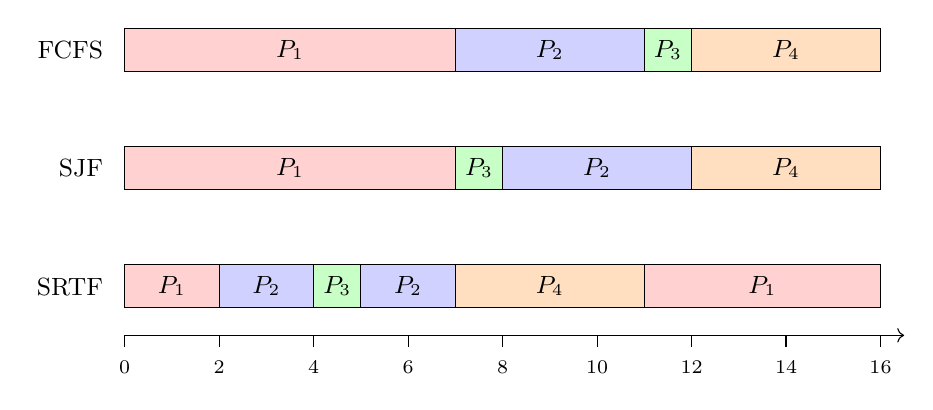
\begin{tikzpicture}[font=\small]
    \def\s{0.6}
    % ---- FCFS ----
    \node[anchor=east] at (-0.15,3.27) {FCFS};
    \draw[fill=red!18] (0,3.0) rectangle ({7*\s},3.55);
    \node at ({3.5*\s},3.275) {$P_1$};
    \draw[fill=blue!18] ({7*\s},3.0) rectangle ({11*\s},3.55);
    \node at ({9*\s},3.275) {$P_2$};
    \draw[fill=green!22] ({11*\s},3.0) rectangle ({12*\s},3.55);
    \node at ({11.5*\s},3.275) {$P_3$};
    \draw[fill=orange!25] ({12*\s},3.0) rectangle ({16*\s},3.55);
    \node at ({14*\s},3.275) {$P_4$};
    % ---- SJF ----
    \node[anchor=east] at (-0.15,1.77) {SJF};
    \draw[fill=red!18] (0,1.5) rectangle ({7*\s},2.05);
    \node at ({3.5*\s},1.775) {$P_1$};
    \draw[fill=green!22] ({7*\s},1.5) rectangle ({8*\s},2.05);
    \node at ({7.5*\s},1.775) {$P_3$};
    \draw[fill=blue!18] ({8*\s},1.5) rectangle ({12*\s},2.05);
    \node at ({10*\s},1.775) {$P_2$};
    \draw[fill=orange!25] ({12*\s},1.5) rectangle ({16*\s},2.05);
    \node at ({14*\s},1.775) {$P_4$};
    % ---- SRTF ----
    \node[anchor=east] at (-0.15,0.27) {SRTF};
    \draw[fill=red!18] (0,0) rectangle ({2*\s},0.55);
    \node at ({1*\s},0.275) {$P_1$};
    \draw[fill=blue!18] ({2*\s},0) rectangle ({4*\s},0.55);
    \node at ({3*\s},0.275) {$P_2$};
    \draw[fill=green!22] ({4*\s},0) rectangle ({5*\s},0.55);
    \node at ({4.5*\s},0.275) {$P_3$};
    \draw[fill=blue!18] ({5*\s},0) rectangle ({7*\s},0.55);
    \node at ({6*\s},0.275) {$P_2$};
    \draw[fill=orange!25] ({7*\s},0) rectangle ({11*\s},0.55);
    \node at ({9*\s},0.275) {$P_4$};
    \draw[fill=red!18] ({11*\s},0) rectangle ({16*\s},0.55);
    \node at ({13.5*\s},0.275) {$P_1$};
    % ---- 时间轴 ----
    \draw[->] (0,-0.35) -- ({16*\s+0.3},-0.35);
    \foreach \x in {0,2,4,6,8,10,12,14,16} {
        \draw (\x*\s,-0.35) -- (\x*\s,-0.5);
        \node[font=\scriptsize] at (\x*\s,-0.75) {\x};
    }
\end{tikzpicture}
\caption{FCFS / SJF / SRTF 甘特图（同一进程集合，时间单位）}
\end{figure}

\begin{table}[H]
\centering
\caption{三种非交互算法对比}
\begin{tabulary}{\textwidth}{CCCC}
\toprule
算法 & 抢占 & 平均周转 & 平均等待 \\
\midrule
FCFS & 否 & 8.75 & 4.75 \\
SJF  & 否 & 8.00 & 4.00 \\
SRTF & 是 & 7.00 & 3.00 \\
\bottomrule
\end{tabulary}
\end{table}

\noindent SRTF 的指标最好，但抢占带来更多上下文切换；且三者都以「长作业饥饿」为代价换取短作业的响应。SJF/SRTF 的理论最优性依赖运行时间可预知，实际系统只能用历史行为估计。

\section{时间片轮转 RR 与优先级调度}

\subsection{时间片轮转 RR}

RR 为每个进程分配一个固定时间片 $q$，就绪队列按 \textbf{FIFO 轮转}：进程用完一个时间片即被抢占并排到队尾；若在时间片内完成或主动阻塞则提前让出。RR \textbf{抢占}且天然公平，是分时系统的基石。

取与上表相同运行时间但\textbf{同时到达}的进程，$q=2$：序列为
\[
P_1[0,2] \to P_2[2,4] \to P_3[4,5] \to P_4[5,7] \to P_1[7,9] \to P_2[9,11] \to P_4[11,13] \to P_1[13,16]
\]
完成时刻 $c=(16,11,5,13)$，于是
\begin{equation}
    \overline{T_{\text{周转}}} = \frac{16+11+5+13}{4} = 11.25,\qquad
    \overline{T_{\text{等待}}} = \frac{9+7+4+9}{4} = 7.25,\qquad
    \overline{T_{\text{响应}}} = \frac{0+2+4+5}{4} = 2.75
\end{equation}

\begin{figure}[H]
\centering
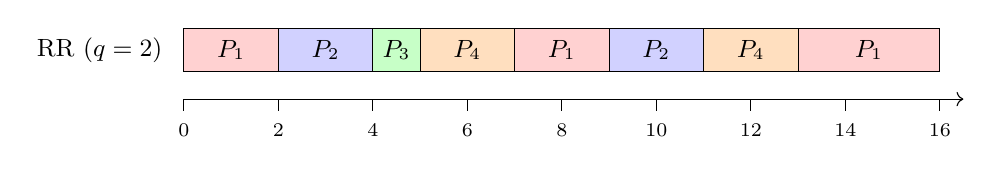
\begin{tikzpicture}[font=\small]
    \def\s{0.6}
    \node[anchor=east] at (-0.15,1.27) {RR ($q=2$)};
    \draw[fill=red!18] (0,1.0) rectangle ({2*\s},1.55);
    \node at ({1*\s},1.275) {$P_1$};
    \draw[fill=blue!18] ({2*\s},1.0) rectangle ({4*\s},1.55);
    \node at ({3*\s},1.275) {$P_2$};
    \draw[fill=green!22] ({4*\s},1.0) rectangle ({5*\s},1.55);
    \node at ({4.5*\s},1.275) {$P_3$};
    \draw[fill=orange!25] ({5*\s},1.0) rectangle ({7*\s},1.55);
    \node at ({6*\s},1.275) {$P_4$};
    \draw[fill=red!18] ({7*\s},1.0) rectangle ({9*\s},1.55);
    \node at ({8*\s},1.275) {$P_1$};
    \draw[fill=blue!18] ({9*\s},1.0) rectangle ({11*\s},1.55);
    \node at ({10*\s},1.275) {$P_2$};
    \draw[fill=orange!25] ({11*\s},1.0) rectangle ({13*\s},1.55);
    \node at ({12*\s},1.275) {$P_4$};
    \draw[fill=red!18] ({13*\s},1.0) rectangle ({16*\s},1.55);
    \node at ({14.5*\s},1.275) {$P_1$};
    \draw[->] (0,0.65) -- ({16*\s+0.3},0.65);
    \foreach \x in {0,2,4,6,8,10,12,14,16} {
        \draw (\x*\s,0.65) -- (\x*\s,0.5);
        \node[font=\scriptsize] at (\x*\s,0.25) {\x};
    }
\end{tikzpicture}
\caption{RR 甘特图（时间片 $q=2$，进程同时到达）}
\end{figure}

\subsection{时间片大小的影响}

时间片 $q$ 是 RR 最重要的参数，直接决定「响应性」与「切换开销」的折中：

\begin{itemize}
    \item $q \to \infty$：RR 退化为 FCFS，响应时间变差，但切换最少。
    \item $q \to 0$：每个指令都切换，上下文切换开销吞掉有效计算，吞吐量骤降。
    \item $q$ 应略大于「一次上下文切换时间」且覆盖绝大多数 CPU 突发，经验上取 $10\sim100$ ms。
\end{itemize}

对同一集合（同时到达）计算不同 $q$（切换开销忽略）：

\begin{table}[H]
\centering
\caption{时间片 $q$ 对指标的影响（同时到达）}
\begin{tabulary}{\textwidth}{CCCC}
\toprule
时间片 $q$ & 平均等待 & 平均响应 & 平均周转 \\
\midrule
1 & 7.00 & 1.50 & 11.00 \\
2 & 7.25 & 2.75 & 11.25 \\
4 & 7.50 & 5.25 & 11.50 \\
$\infty$ (FCFS) & 7.50 & 7.50 & 11.50 \\
\bottomrule
\end{tabulary}
\end{table}

\noindent 结论：在上例中总完成时间恒为 16（单 CPU、不空闲），但\textbf{时间片越小，响应越快}（首轮轮转更早到达每个进程），代价是切换更频繁；时间片越大越接近 FCFS。因此 $q$ 的选取要在响应时间与吞吐量之间折中。

\subsection{优先级调度}

每个进程赋予一个优先级，调度器总是选择\textbf{优先级最高}的就绪进程。约定数值越小优先级越高。优先级可\textbf{静态}给定，也可\textbf{动态}调整。主要问题有二：

\begin{itemize}
    \item \textbf{饥饿 (starvation)}：低优先级进程可能长期得不到 CPU。
    \item \textbf{优先级反转 (priority inversion)}：低优先级进程持有高优先级进程所需的锁，导致后者被中优先级进程阻塞，可用优先级继承缓解。
\end{itemize}

对同时到达、优先级为 $P_2(1)>P_4(2)>P_1(3)>P_3(4)$ 的集合做非抢占优先级调度，序列为
\[
P_2[0,4] \to P_4[4,8] \to P_1[8,15] \to P_3[15,16]
\]
\begin{equation}
    \overline{T_{\text{周转}}} = \frac{15+4+16+8}{4} = 10.75,\qquad
    \overline{T_{\text{等待}}} = \frac{8+0+15+4}{4} = 6.75
\end{equation}

\begin{figure}[H]
\centering
\begin{tikzpicture}[font=\small]
    \def\s{0.6}
    \node[anchor=east] at (-0.15,0.27) {优先级};
    \draw[fill=blue!18] (0,0) rectangle ({4*\s},0.55);
    \node at ({2*\s},0.275) {$P_2$};
    \draw[fill=orange!25] ({4*\s},0) rectangle ({8*\s},0.55);
    \node at ({6*\s},0.275) {$P_4$};
    \draw[fill=red!18] ({8*\s},0) rectangle ({15*\s},0.55);
    \node at ({11.5*\s},0.275) {$P_1$};
    \draw[fill=green!22] ({15*\s},0) rectangle ({16*\s},0.55);
    \node at ({15.5*\s},0.275) {$P_3$};
    \draw[->] (0,-0.35) -- ({16*\s+0.3},-0.35);
    \foreach \x in {0,2,4,6,8,10,12,14,16} {
        \draw (\x*\s,-0.35) -- (\x*\s,-0.5);
        \node[font=\scriptsize] at (\x*\s,-0.75) {\x};
    }
\end{tikzpicture}
\caption{非抢占优先级调度甘特图（数值小者优先）}
\end{figure}

\noindent RR 与优先级的结合即\textbf{优先级 + 时间片}：高优先级队列内轮转，既保响应又防独占。

\section{多级反馈队列 MLFQ}

MLFQ 不要求预知运行时间，而是用「多个优先级队列 + 反馈」动态推测进程类型（CPU 密集型还是 I/O 密集型）。核心规则：

\begin{enumerate}
    \item \textbf{多队列、优先级递减}：设 $Q_0,Q_1,\dots,Q_{n-1}$，$Q_0$ 优先级最高。总是调度最高优先级非空队列中的进程。
    \item \textbf{时间片随层级递增}：高优先级队列用短时间片（如 $Q_0$ 为 2），低优先级队列用长时间片（如 $Q_1$ 为 4，$Q_2$ 为 FCFS），以适配不同进程。
    \item \textbf{新进程入最高队列}：所有新进程先进入 $Q_0$，享受最短响应。
    \item \textbf{用完整个时间片则降级}：进程若耗尽分配的整个时间片仍未完成，说明偏 CPU 密集，被降到下一级队列。
    \item \textbf{主动让出则保持/升级}：进程在时间片用完前主动让出（如等待 I/O），说明偏交互式，留在原队列（或提升），从而持续获得好响应。
    \item \textbf{周期提升 (priority boost)}：每隔固定时间 $S$，把所有进程重新提到 $Q_0$，防止长作业饥饿，并校正对 CPU/IO 类型的误判。
    \item \textbf{同队列内轮转}：同一优先级队列内部按 RR 调度。
\end{enumerate}

\begin{table}[H]
\centering
\caption{MLFQ 队列参数（示例）}
\begin{tabulary}{\textwidth}{CCCC}
\toprule
队列 & 优先级 & 时间片 & 典型对象 \\
\midrule
$Q_0$ & 最高 & 2 & 新进程、交互式 (I/O 密集) \\
$Q_1$ & 中 & 4 & 短批处理 \\
$Q_2$ & 最低 & FCFS & CPU 密集型长作业 \\
\bottomrule
\end{tabulary}
\end{table}

\noindent MLFQ 用「降级惩罚 CPU 密集、保留奖励 I/O 密集、周期提升兜底饥饿」三条机制，在无需预知运行时间的前提下同时兼顾响应时间与吞吐量，是通用操作系统最常用的调度框架之一。

\clearpage
\clearpage
\begingroup
\let\clearpage\relax
\let\cleardoublepage\relax
\vspace*{\fill}
\chapter{同步与并发}
\begin{center}
多个进程或线程并发访问共享资源时会产生竞态，同步机制用于保证结果的可再现与正确性。本章从临界区问题的三个必要条件出发，依次介绍 Peterson 算法、信号量（P/V）与生产者-消费者、读者-写者问题、管程与条件变量，最后讨论死锁的四个必要条件、资源分配图与银行家算法。
\end{center}
\vspace*{\fill}
\endgroup
\clearpage

\section{临界区问题}

多个进程并发访问共享数据，执行的相对顺序不确定，其最终结果依赖于调度时序，这种现象称为\textbf{竞态条件 (race condition)}。把访问共享资源的代码称为\textbf{临界区 (critical section)}。

\subsection{三个必要条件}

任何正确的临界区解决方案必须同时满足以下三个条件。

\begin{table}[H]
\centering
\caption{临界区问题的三个必要条件}
\begin{tabulary}{\textwidth}{LLL}
\toprule
条件 & 含义 & 反例 \\
\midrule
互斥 (Mutual Exclusion) & 任一时刻至多一个进程处于临界区 & 两进程同时写同一变量 \\
前进 (Progress) & 临界区空闲且有进程想进入时，能及时选出进入者，不被无关进程无限阻塞 & 只剩空闲却无人能进 \\
有限等待 (Bounded Waiting) & 一个进程发出进入请求后，在它之前允许其他进程进入的次数有上界 & 某进程被无限插队饿死 \\
\bottomrule
\end{tabulary}
\end{table}

\begin{equation}
    \text{互斥} \ \wedge\ \text{前进} \ \wedge\ \text{有限等待} \;\Longrightarrow\; \text{正确同步}
\end{equation}

仅靠「标志数组」或「轮转」单独使用都无法同时满足三条件：纯标志会互相礼让导致死锁，纯轮转虽保证互斥却违反前进。

\subsection{Peterson 算法}

Peterson 算法是满足三条件的经典软件方案，适用于两个进程。它组合了「意愿标志 \texttt{flag}」与「轮转变量 \texttt{turn}」，其中 \texttt{turn} 用于打破对称僵局。

\begin{lstlisting}[language=C, caption={Peterson 算法（进程 $i$，对方为 $j = 1-i$）}]
flag[i] = true;          // 声明我想进入临界区
turn = j;                // 但先把机会让给对方
while (flag[j] && turn == j) { /* 忙等待 */ }

/* ----- 临界区 ----- */

flag[i] = false;         // 退出后撤销意愿
/* ----- 剩余区 ----- */
\end{lstlisting}

\begin{enumerate}
    \item 置 \texttt{flag[i]=true}，表明进程 $i$ 有进入意图。
    \item 置 \texttt{turn=j}，把优先权交给对方。当两者同时竞争时，\texttt{turn} 的最后一次写入决定了谁等待。
    \item 循环等待：只要对方也想进入且 \texttt{turn} 指向对方，就让其先进入。
    \item 进入临界区，执行完后置 \texttt{flag[i]=false}，允许对方进入。
\end{enumerate}

\textbf{正确性}：若两进程同时进入 while，则 \texttt{turn} 只能取一个值，其中一方必然满足 \texttt{turn != j} 而跳出，保证\textbf{互斥}；退出者一旦置 \texttt{flag=false}，等待者即可进入，满足\textbf{前进}；对方至多进入一次后 \texttt{turn} 被改写，满足\textbf{有限等待}。但 Peterson 依赖顺序一致的内存模型，在多核弱一致内存上需内存屏障。

\section{信号量}

\subsection{P/V 操作}

信号量 $S$ 是一个受保护的整型变量，只能通过两个\emph{原子}操作访问：

\begin{lstlisting}[language=C, caption={信号量的 wait (P) 与 signal (V)}]
wait(S):            // P 操作 / 申请资源，可能阻塞
    S.value--;      // 也可写为 while (S.value <= 0) ;
    if (S.value < 0)
        block();    // 无资源则入等待队列

signal(S):          // V 操作 / 释放资源，可唤醒等待者
    S.value++;
    if (S.value <= 0)
        wakeup();   // 尚有等待者，唤醒其一
\end{lstlisting}

\begin{itemize}
    \item \textbf{二元信号量 (binary semaphore)}：取值仅 $\{0,1\}$，退化为互斥锁，用于临界区互斥。
    \item \textbf{计数信号量 (counting semaphore)}：取值为非负整数 $n$，表示可用资源数量，初值即资源总数。
\end{itemize}

P、V 必须成对出现；P 阻塞调用者，V 唤醒一个等待者。若把 P/V 原子性破坏，互斥就会失效。

\subsection{生产者-消费者问题}

设缓冲区容量为 $n$，信号量 \texttt{mutex} 保护缓冲区本身的互斥访问，\texttt{empty}、\texttt{full} 分别表示空槽与满槽数量。

\begin{lstlisting}[language=C, caption={生产者-消费者（有限缓冲区）}]
semaphore mutex = 1;   // 缓冲区互斥
semaphore empty = n;   // 空槽数
semaphore full  = 0;   // 满槽数

producer():                       consumer():
    while (true) {                    while (true) {
        item = produce();                 wait(full);    // 等待有产品
        wait(empty);    // 等空槽          wait(mutex);   // 进入临界区
        wait(mutex);    // 进入临界区      item = take();  // 取走并腾出
        put(item);                        signal(mutex);
        signal(mutex);                    signal(empty); // 空槽 +1
        signal(full);   // 产品数 +1      consume(item);
    }                                 }
\end{lstlisting}

\textbf{顺序要点}：必须先 \texttt{wait(empty)} 再 \texttt{wait(mutex)}。若颠倒，生产者可能持有 \texttt{mutex} 却在 \texttt{empty} 上阻塞，消费者无法进入而永久等待，形成死锁。

\subsection{读者-写者问题}

允许多个读者同时读，但写者必须独占。第一类（读者优先）可能使写者饥饿；第二类（写者优先）可能使读者饥饿。

\begin{lstlisting}[language=C, caption={读者-写者（读者优先）}]
semaphore rw_mutex = 1;  // 读写的互斥锁
semaphore mutex    = 1;  // 保护 read_count
int read_count = 0;

reader():                              writer():
    wait(mutex);                           wait(rw_mutex);
    read_count++;                          /* 写操作 */
    if (read_count == 1) wait(rw_mutex);   signal(rw_mutex);
    signal(mutex);
    /* 读操作 */
    wait(mutex);
    read_count--;
    if (read_count == 0) signal(rw_mutex);
    signal(mutex);
\end{lstlisting}

\section{管程与条件变量}

管程 (monitor) 是把共享变量和操作它们的过程封装在一起的高级同步抽象：任一时刻只允许一个进程在管程内活动，互斥由编译器/运行库隐式保证，无需手工加锁。管程内用\textbf{条件变量}实现等待与唤醒。

\begin{table}[H]
\centering
\caption{管程内条件变量的操作}
\begin{tabulary}{\textwidth}{LLL}
\toprule
操作 & 语义 & 说明 \\
\midrule
\texttt{c.wait()} & 释放管程锁并阻塞于条件 $c$ & 被唤醒后须重新获得管程锁才返回 \\
\texttt{c.signal()} & 唤醒一个等待 $c$ 的进程 & 若无等待者则该调用无效果 \\
\bottomrule
\end{tabulary}
\end{table}

\begin{lstlisting}[language=C, caption={管程实现生产者-消费者}]
monitor BoundedBuffer {
    item buf[n]; int count = 0;
    condition notFull, notEmpty;   // 条件变量

    void produce(item x) {
        if (count == n) notFull.wait();   // 满则等待
        buf[in] = x; in = (in + 1) % n; count++;
        notEmpty.signal();                // 唤醒等待的消费者
    }
    item consume() {
        if (count == 0) notEmpty.wait();  // 空则等待
        item x = buf[out]; out = (out + 1) % n; count--;
        notFull.signal();                 // 唤醒等待的生产者
        return x;
    }
}
\end{lstlisting}

条件变量与信号量不同：信号量有计数值并可跨进程传递状态，而 \texttt{signal} 只在已有等待者时才生效，且不保存「许可」。因此需用 \texttt{while} 而非 \texttt{if} 重新检查条件（Mesa 语义下可能虚假唤醒）。

\section{死锁}

\subsection{四个必要条件}

死锁 (deadlock) 指一组进程因互相等待对方持有的资源而永久阻塞。四个条件必须\emph{同时}成立才可能死锁；破坏任一条件即可预防。

\begin{table}[H]
\centering
\caption{死锁的四个必要条件}
\begin{tabulary}{\textwidth}{LLL}
\toprule
条件 & 含义 & 破坏策略 \\
\midrule
互斥 (Mutual Exclusion) & 资源一次只能被一个进程占用 & 尽量共享（如只读文件） \\
占有并等待 (Hold and Wait) & 持有资源的同时等待新资源 & 一次性申请全部资源 \\
不可抢占 (No Preemption) & 资源只能被持有者主动释放 & 允许抢占、回滚 \\
循环等待 (Circular Wait) & 存在进程-资源的环形等待链 & 给资源编号，按序申请 \\
\bottomrule
\end{tabulary}
\end{table}

\subsection{资源分配图}

资源分配图用有向图描述时刻状态：圆形表示进程 $P$，方形表示资源 $R$（内部黑点表示实例数）。$P \to R$ 为\textbf{请求边}，$R \to P$ 为\textbf{分配边}。图中出现\emph{环}是死锁的必要条件：单实例时环即死锁；多实例时环只是可能死锁，还需结合可用实例判断。

\begin{figure}[H]
\centering
\begin{tikzpicture}[font=\small, >=stealth, node distance=1.5cm]
    % 资源
    \node[draw, rectangle, fill=orange!12, minimum size=1cm] (r1) {$R_1$};
    \node[draw, rectangle, fill=orange!12, minimum size=1cm, right=3cm of r1] (r2) {$R_2$};
    \fill (r1.center) ++(-0.18,0) circle (2pt);
    \fill (r2.center) ++(0,0) circle (2pt);
    \fill (r2.center) ++(0.22,0) circle (2pt);
    % 进程
    \node[draw, circle, fill=blue!8] (p1) at ($(r1)+(0,-3)$) {$P_1$};
    \node[draw, circle, fill=blue!8] (p2) at ($(r2)+(0,-3)$) {$P_2$};
    % 分配: R1 -> P1 ; R2 -> P2
    \draw[->] (r1) -- (p1);
    \draw[->] (r2) -- (p2);
    % 请求: P1 -> R2 ; P2 -> R1
    \draw[->] (p1) to[bend left=15] (r2);
    \draw[->] (p2) to[bend left=15] (r1);
    \node[font=\footnotesize, below=0.2cm of p1] {持有 $R_1$、请求 $R_2$};
    \node[font=\footnotesize, below=0.2cm of p2] {持有 $R_2$、请求 $R_1$};
\end{tikzpicture}
\caption{资源分配图：$P_1$ 与 $P_2$ 互相请求对方持有的资源，形成环}
\end{figure}

\subsection{银行家算法}

银行家算法在进程提出资源请求时进行\textbf{安全性检查}：若分配后系统仍处于安全状态则满足请求，否则推迟，从而避免死锁。

\begin{align}
    Need[i] &= Max[i] - Allocation[i] \\
    Available' &= Available + Allocation[i] \quad (\text{当 } Need[i] \le Available)
\end{align}

\begin{algorithm}[H]
\caption{银行家算法：安全性检查}
\begin{algorithmic}[1]
\State 令 $Work = Available$，$Finish[i] = \text{false}\ (i=1,\dots,n)$
\While{存在 $i$ 使 $Finish[i]=\text{false}$ 且 $Need[i] \le Work$}
    \State $Work \gets Work + Allocation[i]$
    \State $Finish[i] \gets \text{true}$
    \State \textbf{输出} $i$（加入安全序列）
\EndWhile
\If{所有 $Finish[i]=\text{true}$}
    \State \Return \textbf{安全}，安全序列即输出顺序
\Else
    \State \Return \textbf{不安全}（可能死锁）
\EndIf
\end{algorithmic}
\end{algorithm}

\noindent 以经典例子 $Available=(3,3,2)$ 说明：

\begin{table}[H]
\centering
\caption{银行家算法示例（资源类型 $A,B,C$）}
\begin{tabulary}{\textwidth}{CCCCC}
\toprule
进程 & $Max$ & $Allocation$ & $Need$ & 完成顺序 \\
\midrule
$P_0$ & (7,5,3) & (0,1,0) & (7,4,3) & 4 \\
$P_1$ & (3,2,2) & (2,0,0) & (1,2,2) & 1 \\
$P_2$ & (9,0,2) & (3,0,2) & (6,0,0) & 5 \\
$P_3$ & (2,2,2) & (2,1,1) & (0,1,1) & 2 \\
$P_4$ & (4,3,3) & (0,0,2) & (4,3,1) & 3 \\
\bottomrule
\end{tabulary}
\end{table}

检查过程：$Need[P_1]=(1,2,2)\le(3,3,2)$，完成后 $Work=(5,3,2)$；$Need[P_3]=(0,1,1)\le Work$，$Work=(7,4,3)$；$Need[P_4]=(4,3,1)\le Work$，$Work=(7,4,5)$；$Need[P_0]=(7,4,3)\le Work$，$Work=(7,5,5)$；最后 $Need[P_2]=(6,0,0)\le Work$ 完成。

\begin{equation}
    \text{安全序列：}\ P_1 \to P_3 \to P_4 \to P_0 \to P_2
\end{equation}

存在安全序列说明系统当前安全，即使各进程按此顺序依次申请，也能全部完成；否则系统进入不安全状态，应采用资源预分配、避免或恢复（抢占、回滚、终止进程）等策略。

\clearpage
\clearpage
\begingroup
\let\clearpage\relax
\let\cleardoublepage\relax
\vspace*{\fill}
\chapter{内存管理}
\begin{center}
内存管理解决「多个程序如何共享有限物理内存」的问题：通过逻辑地址与物理地址的分离、重定位与保护机制，为每个进程提供独立地址空间；再以分页、分段及其组合把连续的虚拟地址映射到离散的物理帧，并用 TLB 与多级页表控制平均访存开销。
\end{center}
\vspace*{\fill}
\endgroup
\clearpage

\section{地址空间与重定位}

\subsection{逻辑地址与物理地址}

\begin{itemize}
    \item \textbf{逻辑地址（虚拟地址）}：CPU 生成的地址，面向进程视角，从 0 开始连续编号。
    \item \textbf{物理地址}：内存单元的真实地址，由内存总线送入存储体。
    \item 二者关系由内存管理单元在运行时完成转换；编译期只能确定逻辑地址。
\end{itemize}

地址绑定可在三个时机发生：

\begin{table}[H]
\centering
\caption{地址绑定的时机}
\begin{tabulary}{\textwidth}{LLL}
\toprule
时机 & 说明 & 特点 \\
\midrule
编译时 & 生成绝对地址代码 & 程序位置固定，重定位需重新编译 \\
装入时 & 装入时把逻辑地址改写为物理地址 & 一旦装入不能移动 \\
执行时 & 运行时由 MMU 动态重定位 & 灵活，支持换入换出与虚拟内存 \\
\bottomrule
\end{tabulary}
\end{table}

\subsection{MMU 与基址/界限寄存器}

内存管理单元（MMU）是 CPU 与内存之间的硬件，负责把逻辑地址翻译成物理地址并实施保护。最朴素的重定位方案为每个进程维护一对寄存器：

\begin{itemize}
    \item \textbf{基址寄存器 (base)}：进程可用物理内存的起始地址。
    \item \textbf{界限寄存器 (limit)}：进程地址空间的长度。
\end{itemize}

\begin{equation}
    \text{物理地址} = \text{base} + \text{逻辑地址}, \qquad
    \text{合法} \iff 0 \le \text{逻辑地址} < \text{limit}
\end{equation}

若逻辑地址越过 limit，则触发越界陷阱（trap），交由内核处理，从而实现进程间的存储保护。

\begin{figure}[H]
\centering
\begin{tikzpicture}[font=\small, >=stealth, node distance=1.2cm]
    \node[draw, rounded corners, fill=blue!8, minimum width=3.2cm] (cpu) {CPU};
    \node[draw, rounded corners, fill=gray!10, right=2.2cm of cpu, minimum width=3.4cm, align=center] (mmu) {MMU\\ \scriptsize base / limit};
    \node[draw, rounded corners, fill=green!10, right=2.2cm of mmu, minimum width=3.4cm, align=center] (mem) {内存\\ \scriptsize 物理地址空间};
    \draw[->] (cpu) -- node[above]{\scriptsize 逻辑地址} (mmu);
    \draw[->] (mmu) -- node[above]{\scriptsize 物理地址} (mem);
    \draw[->] (mem) to[bend left=35] (cpu);
    \draw[->, red] (mmu) to[bend right=35] node[below]{\scriptsize 越界陷阱} (cpu);
\end{tikzpicture}
\caption{MMU 在逻辑地址与物理地址之间完成重定位}
\end{figure}

\section{分页}

\subsection{页、帧与页表}

分页把逻辑地址空间切成大小相等的\textbf{页 (page)}，把物理内存切成同样大小的\textbf{帧 (frame)}。页与帧大小相同且为 2 的幂（如 4\,KB），页可以装入任意空闲帧，从而消除外部碎片。

页表（page table）为每个进程建立「页号 $\to$ 帧号」的映射，通常存放在内存中。

\begin{equation}
    \text{逻辑地址} = \underbrace{p}_{\text{页号}} \;\|\; \underbrace{d}_{\text{页内偏移}}, \qquad
    p = \left\lfloor \frac{LA}{S} \right\rfloor,\quad d = LA \bmod S
\end{equation}

\begin{equation}
    PA = f \times S + d, \qquad f = \text{页表}[p]
\end{equation}

其中 $S$ 为页大小，$f$ 为页号 $p$ 对应的帧号。由于 $S$ 是 2 的幂，除以 $S$ 等价于右移 $\log_2 S$ 位，取模等价于取低 $\log_2 S$ 位，因此地址翻译可完全由位切分实现。

\begin{figure}[H]
\centering
\begin{tikzpicture}[font=\small, >=stealth]
    \draw (0,0) rectangle (2,0.8) node[midway] {$p$};
    \draw (2,0) rectangle (4,0.8) node[midway] {$d$};
    \node at (1,-0.42) {\scriptsize 页号};
    \node at (3,-0.42) {\scriptsize 偏移};
    \node[above] at (2,0.85) {\scriptsize 逻辑地址};

    \node[draw, rounded corners, fill=blue!8, minimum width=2.0cm, minimum height=1.4cm, align=center] (pt) at (5.6,0.4) {页表\\[2pt] \scriptsize $p \Rightarrow f$};
    \draw[->] (2,0.6) -- (pt.west);

    \draw (8,0) rectangle (9.4,0.8) node[midway] {$f$};
    \draw (9.4,0) rectangle (11.4,0.8) node[midway] {$d$};
    \node at (8.7,-0.42) {\scriptsize 帧号};
    \node at (10.4,-0.42) {\scriptsize 偏移};
    \node[above] at (9.7,0.85) {\scriptsize 物理地址};
    \draw[->] (pt.east) -- (8,0.6);
\end{tikzpicture}
\caption{分页地址翻译：页号查页表得帧号，偏移原样保留}
\end{figure}

\subsection{页表项 PTE}

页表项（Page Table Entry）除帧号外还记录若干控制位：

\begin{table}[H]
\centering
\caption{页表项的主要字段}
\begin{tabulary}{\textwidth}{LLL}
\toprule
字段 & 位宽 & 作用 \\
\midrule
帧号 (frame number) & 视物理内存大小而定 & 该页映射到的物理帧 \\
有效位 (valid / present) & 1 & 页面是否已装入内存，0 触发缺页 \\
修改位 (dirty) & 1 & 页面是否被写过，决定换出时是否回写 \\
访问位 (reference) & 1 & 是否被访问，供置换算法参考 \\
保护位 (protection) & 2--3 & 读/写/执行权限，越权触发保护异常 \\
\bottomrule
\end{tabulary}
\end{table}

在 32 位、4\,KB 页的单级页表下，需要 $2^{20}$ 个表项、约 4\,MB，且每个进程一份。为压缩开销引入\textbf{多级页表}：只把用到的下级页表装入内存，未用的页目录项置空，从而大幅节省空间。

\begin{equation}
    \text{逻辑地址} = \underbrace{p_1}_{\text{页目录}} \;\|\; \underbrace{p_2}_{\text{页表}} \;\|\; \underbrace{d}_{\text{偏移}}
\end{equation}

\section{分段}

\subsection{段表与保护}

分段按程序的逻辑结构（代码段、数据段、栈段）把地址空间划分为长度可变的\textbf{段 (segment)}。每个进程一张\textbf{段表}，表项含段的\textbf{基址 base} 与\textbf{界限 limit}。

\begin{equation}
    \text{逻辑地址} = \underbrace{s}_{\text{段号}} \;\|\; \underbrace{d}_{\text{段内偏移}}, \qquad
    \text{合法} \iff d < \text{limit}[s],\qquad PA = \text{base}[s] + d
\end{equation}

若 $d \ge \text{limit}[s]$ 则触发越界异常，实现按段的保护与共享。

\begin{figure}[H]
\centering
\begin{tikzpicture}[font=\small, >=stealth]
    \node[draw, rounded corners, fill=blue!8, minimum width=3.4cm, minimum height=2.4cm, align=center] (st) {段表\\[3pt] \scriptsize 段号 $s$\\ \scriptsize base$[s]$ \quad limit$[s]$};
    \node[left=1.8cm of st, align=center] (la) {逻辑地址\\ \scriptsize $s \,\|\, d$};
    \draw[->] (la) -- (st);
    \node[right=1.8cm of st, align=center] (pa) {物理地址\\ \scriptsize $base[s]+d$};
    \draw[->] (st) -- node[above, yshift=2pt]{\scriptsize $d<\text{limit}[s]$?} (pa);
    \draw[->, red] (st.south) -- ++(0,-0.9) node[below]{\scriptsize $d\ge\text{limit}$：越界异常};
\end{tikzpicture}
\caption{分段地址翻译与越界检查}
\end{figure}

\subsection{分段与分页对比}

\begin{table}[H]
\centering
\caption{分页与分段的对比}
\begin{tabulary}{\textwidth}{LLL}
\toprule
维度 & 分页 & 分段 \\
\midrule
划分依据 & 物理等分为固定大小的页 & 按逻辑结构划分为变长段 \\
大小 & 固定（页 = 帧） & 可变 \\
地址结构 & 一维：页号 + 偏移 & 二维：段号 + 偏移 \\
碎片 & 仅内部碎片 & 仅外部碎片 \\
对用户 & 透明 & 可见，便于共享与保护 \\
\bottomrule
\end{tabulary}
\end{table}

\subsection{段页式}

段页式结合二者：先按逻辑分段，再把每段分页装入物理帧。逻辑地址为三维结构。

\begin{equation}
    \text{逻辑地址} = \underbrace{s}_{\text{段号}} \;\|\; \underbrace{p}_{\text{页号}} \;\|\; \underbrace{d}_{\text{页内偏移}}
\end{equation}

翻译路径：段表$[s]$ 得该段的页表 $\to$ 页表$[p]$ 得帧号 $f$ $\to$ $PA = f \times S + d$。段页式既保留分段的逻辑与保护，又消除外部碎片；代价是需要多次访存，通常由 TLB 加速。

\section{TLB 与有效访问时间 EAT}

\subsection{快表 TLB}

页表在内存中，若每次访存都先查页表会使访问次数翻倍。\textbf{转换检测缓冲区 (TLB)} 是一块高速相联存储器，缓存最近使用的「页号 $\to$ 帧号」表项。

\begin{itemize}
    \item \textbf{TLB 命中}：直接得到帧号，与偏移拼接得物理地址，无需访存页表。
    \item \textbf{TLB 缺失}：访问内存中的页表（可能多级）取帧号，并更新 TLB。
\end{itemize}

\begin{figure}[H]
\centering
\begin{tikzpicture}[font=\small, >=stealth, node distance=1.15cm,
    box/.style={draw, rounded corners, minimum width=3.6cm, minimum height=0.8cm, align=center}]
    \node[box, fill=blue!8] (cpu) {CPU 逻辑地址};
    \node[box, fill=yellow!20, below=of cpu] (tlb) {查 TLB};
    \node[box, fill=green!12, below=of tlb] (hit) {命中：取帧号};
    \node[box, fill=orange!15, below=of hit] (miss) {缺失：访存查页表};
    \node[box, fill=gray!12, below=of miss] (pa) {物理地址};
    \draw[->] (cpu) -- (tlb);
    \draw[->] (tlb) -- node[right]{\scriptsize hit} (hit);
    \draw[->] (tlb.east) to[bend left=40] node[right]{\scriptsize miss} (miss.east);
    \draw[->] (hit) -- node[right]{\scriptsize 拼接 $d$} (pa);
    \draw[->] (miss) -- (pa);
    \draw[->] (miss.east) to[bend left=40] node[right]{\scriptsize 回填} (tlb.east);
\end{tikzpicture}
\caption{TLB 的命中与缺失路径}
\end{figure}

\subsection{有效访问时间}

设 TLB 命中率为 $h$，TLB 访问时间为 $t_{\text{TLB}}$，一次内存访问时间为 $t_{\text{mem}}$。命中时只需「查 TLB + 访存数据」，共 $t_{\text{TLB}}+t_{\text{mem}}$；缺失时还需额外一次访存读页表，共 $t_{\text{TLB}}+2t_{\text{mem}}$。

\begin{equation}
    EAT = h\,(t_{\text{TLB}} + t_{\text{mem}}) + (1-h)\,(t_{\text{TLB}} + 2t_{\text{mem}})
        = t_{\text{TLB}} + (2-h)\,t_{\text{mem}}
\end{equation}

若不存在 TLB（每次都查页表），则 $EAT = 2t_{\text{mem}}$。可见 $h \to 1$ 时 $EAT \to t_{\text{TLB}}+t_{\text{mem}}$，接近直接访存的开销。

\begin{table}[H]
\centering
\caption{EAT 随 TLB 命中率的变化（$t_{\text{TLB}}=10$\,ns，$t_{\text{mem}}=100$\,ns）}
\begin{tabulary}{\textwidth}{CCCC}
\toprule
$h$ & 命中路径 (ns) & 未命中路径 (ns) & $EAT$ (ns) \\
\midrule
0.80 & 110 & 210 & 130.0 \\
0.90 & 110 & 210 & 120.0 \\
0.98 & 110 & 210 & 112.0 \\
1.00 & 110 & 210 & 110.0 \\
\bottomrule
\end{tabulary}
\end{table}

\noindent 结论：TLB 命中率每提升一点都会显著降低平均访存时间，因此命中率与 TLB 容量、置换策略密切相关；多级页表虽然省空间，却增加了缺失时的访存次数，二者需与 TLB 配合折中。

\clearpage
\clearpage
\begingroup
\let\clearpage\relax
\let\cleardoublepage\relax
\vspace*{\fill}
\chapter{虚拟内存}
\begin{center}
虚拟内存让每个进程都以为自己独占一整块连续地址空间：它把内存抽象成「按需装入的页」，
用磁盘充当后备存储，并以页面置换让有限的物理帧在多个进程间复用。
本章沿「按需分页 $\to$ 置换策略 $\to$ Belady 异常 $\to$ 抖动与工作集」的主线展开，
重点能用可计算的引用串手算缺页次数。
\end{center}
\vspace*{\fill}
\endgroup
\clearpage

\section{按需分页与缺页处理流程}

虚拟地址被划分为\textbf{页号}与\textbf{页内偏移}，由 MMU 借助页表把页号翻译成物理帧号。
按需分页的核心是：进程启动时并不把全部页调入内存，只有当指令或数据真正被访问、
且对应页不在内存时，才触发\textbf{缺页异常}把页调入。这种「懒惰装入」显著减小了驻留集与启动开销。

\subsection{地址翻译与页表项}

\begin{equation}
    \underbrace{\text{页号 } p}_{v-p \text{ 位}} \;\|\; \underbrace{\text{页内偏移 } d}_{p \text{ 位}}
    \xrightarrow{\ \text{页表}\ } \underbrace{\text{帧号 } f}_{\text{物理地址高位}} \;\|\; d
\end{equation}

页表中的每个页表项（PTE）除了帧号，还要携带若干状态位来支撑按需分页与置换：

\begin{table}[H]
\centering
\caption{页表项的典型字段}
\begin{tabulary}{\textwidth}{LLL}
\toprule
字段 & 含义 & 作用 \\
\midrule
有效位 (valid) & 该页是否在内存 & 为 0 时访问即触发缺页 \\
帧号 (frame) & 物理帧编号 & 地址翻译的结果 \\
脏位 (dirty) & 调入后是否被写过 & 决定换出时是否写回磁盘 \\
访问位 (reference) & 近期是否被访问 & 供 Clock/LRU 近似算法使用 \\
保护位 (protect) & 读/写/执行权限 & 越权访问产生保护异常 \\
\bottomrule
\end{tabulary}
\end{table}

\subsection{缺页处理流程}

触发缺页后，硬件先陷入内核，再由缺页处理程序完成调页。整个流程可概括为六步：
\textbf{trap} $\to$ \textbf{查页表} $\to$ \textbf{判定缺页} $\to$ \textbf{调页入内存} $\to$ \textbf{更新页表} $\to$ \textbf{重新执行指令}。

\begin{figure}[H]
\centering
\begin{tikzpicture}[font=\small, >=stealth, node distance=1.4cm and 2.4cm,
    every node/.style={draw, rounded corners, align=center, fill=blue!6, inner sep=5pt}]
    \node (start) {访问虚拟地址\\MMU 查页表};
    \node[below=of start] (valid) {有效位 $=1$ ?};
    \node[right=of valid, fill=green!12] (hit) {命中\\访问物理帧};
    \node[below=of valid, fill=red!12] (fault) {缺页异常 (trap)};
    \node[below=of fault] (find) {有空闲帧 ?};
    \node[right=of find, fill=orange!15] (load) {调入页面};
    \node[below=of find, fill=orange!15] (victim) {选牺牲页\\脏则写回};
    \node[below=of victim] (update) {更新 PTE / TLB};
    \node[below=of update, fill=green!12] (retry) {重新执行指令};

    \draw[->] (start) -- (valid);
    \draw[->] (valid) -- node[above]{是} (hit);
    \draw[->] (valid) -- node[right]{否} (fault);
    \draw[->] (fault) -- (find);
    \draw[->] (find) -- node[above]{是} (load);
    \draw[->] (find) -- node[right]{否} (victim);
    \draw[->] (load) |- (update);
    \draw[->] (victim) -- (update);
    \draw[->] (update) -- (retry);
    \draw[->, dashed] (retry.west) -- ++(-3.4,0) |- (valid.west);
\end{tikzpicture}
\caption{按需分页的缺页处理流程：查表 $\to$ trap $\to$ 调页 $\to$ 更新 $\to$ 重执行}
\end{figure}

缺页会带来磁盘 I/O，其代价远高于一次内存访问。设缺页率为 $p$，
则\textbf{有效访问时间}（EAT）为内存命中与缺页处理的加权平均：

\begin{equation}
    EAT = (1-p)\, t_{\text{mem}} + p\, t_{\text{fault}},
    \qquad
    p = \frac{F}{N}
\end{equation}

其中 $F$ 为缺页次数，$N$ 为总访问次数。$t_{\text{fault}}$ 通常在毫秒量级，
比 $t_{\text{mem}}$（约百纳秒）大四个数量级，因此\textbf{缺页率哪怕只有百分之几}
都会让性能急剧下降——这正是置换算法与工作集管理要解决的问题。

\section{页面置换算法：FIFO / LRU / 最优 OPT}

物理帧有限，当缺页且无空闲帧时必须\textbf{换出}某一页。选择牺牲页的规则即页面置换算法。
评价指标是给定引用串下的\textbf{缺页次数}。本节以经典引用串 $20$ 次访问为例：

\begin{center}
\texttt{7, 0, 1, 2, 0, 3, 0, 4, 2, 3, 0, 3, 2, 1, 2, 0, 1, 7, 0, 1}
\end{center}

\subsection{三种算法的直觉}

\begin{itemize}
    \item \textbf{FIFO}：淘汰\textbf{最早进入}内存的页，用队列实现；简单，但可能换出仍频繁使用的页，且存在 Belady 异常。
    \item \textbf{LRU}：淘汰\textbf{最久未被使用}的页，符合局部性；需要记录访问时序，硬件完全实现代价高，常用 Clock 近似。
    \item \textbf{OPT}（最优）：淘汰\textbf{未来最长时间不会被访问}的页；缺页次数理论下界，但需预知未来，仅作基准。
\end{itemize}

\subsection{帧数 $=3$ 的逐步模拟}

下表给出三种算法在相同引用串、相同 $3$ 个物理帧下的逐步状态（``—'' 表示空帧）。

\begin{table}[H]
\centering
\caption{FIFO（先进先出），共缺页 $15$ 次}
\begin{tabular}{rrrrrl}
\toprule
步 & 访问页 & 帧1 & 帧2 & 帧3 & 结果 \\
\midrule
 1 & 7 & 7 & — & — & 缺页 \\
 2 & 0 & 7 & 0 & — & 缺页 \\
 3 & 1 & 7 & 0 & 1 & 缺页 \\
 4 & 2 & 2 & 0 & 1 & 缺页（换出 7） \\
 5 & 0 & 2 & 0 & 1 & 命中 \\
 6 & 3 & 2 & 3 & 1 & 缺页（换出 0） \\
 7 & 0 & 2 & 3 & 0 & 缺页（换出 1） \\
 8 & 4 & 4 & 3 & 0 & 缺页（换出 2） \\
 9 & 2 & 4 & 2 & 0 & 缺页（换出 3） \\
10 & 3 & 4 & 2 & 3 & 缺页（换出 0） \\
11 & 0 & 0 & 2 & 3 & 缺页（换出 4） \\
12 & 3 & 0 & 2 & 3 & 命中 \\
13 & 2 & 0 & 2 & 3 & 命中 \\
14 & 1 & 0 & 1 & 3 & 缺页（换出 2） \\
15 & 2 & 0 & 1 & 2 & 缺页（换出 3） \\
16 & 0 & 0 & 1 & 2 & 命中 \\
17 & 1 & 0 & 1 & 2 & 命中 \\
18 & 7 & 7 & 1 & 2 & 缺页（换出 0） \\
19 & 0 & 7 & 0 & 2 & 缺页（换出 1） \\
20 & 1 & 7 & 0 & 1 & 缺页（换出 2） \\
\bottomrule
\end{tabular}
\end{table}

\begin{table}[H]
\centering
\caption{LRU（最近最久未使用），共缺页 $12$ 次}
\begin{tabular}{rrrrrl}
\toprule
步 & 访问页 & 帧1 & 帧2 & 帧3 & 结果 \\
\midrule
 1 & 7 & 7 & — & — & 缺页 \\
 2 & 0 & 7 & 0 & — & 缺页 \\
 3 & 1 & 7 & 0 & 1 & 缺页 \\
 4 & 2 & 2 & 0 & 1 & 缺页（换出 7） \\
 5 & 0 & 2 & 0 & 1 & 命中 \\
 6 & 3 & 2 & 0 & 3 & 缺页（换出 1） \\
 7 & 0 & 2 & 0 & 3 & 命中 \\
 8 & 4 & 4 & 0 & 3 & 缺页（换出 2） \\
 9 & 2 & 4 & 0 & 2 & 缺页（换出 3） \\
10 & 3 & 4 & 3 & 2 & 缺页（换出 0） \\
11 & 0 & 0 & 3 & 2 & 缺页（换出 4） \\
12 & 3 & 0 & 3 & 2 & 命中 \\
13 & 2 & 0 & 3 & 2 & 命中 \\
14 & 1 & 1 & 3 & 2 & 缺页（换出 0） \\
15 & 2 & 1 & 3 & 2 & 命中 \\
16 & 0 & 1 & 0 & 2 & 缺页（换出 3） \\
17 & 1 & 1 & 0 & 2 & 命中 \\
18 & 7 & 1 & 0 & 7 & 缺页（换出 2） \\
19 & 0 & 1 & 0 & 7 & 命中 \\
20 & 1 & 1 & 0 & 7 & 命中 \\
\bottomrule
\end{tabular}
\end{table}

\begin{table}[H]
\centering
\caption{最优置换 OPT，共缺页 $9$ 次（理论下界）}
\begin{tabular}{rrrrrl}
\toprule
步 & 访问页 & 帧1 & 帧2 & 帧3 & 结果 \\
\midrule
 1 & 7 & 7 & — & — & 缺页 \\
 2 & 0 & 7 & 0 & — & 缺页 \\
 3 & 1 & 7 & 0 & 1 & 缺页 \\
 4 & 2 & 2 & 0 & 1 & 缺页（换出 7） \\
 5 & 0 & 2 & 0 & 1 & 命中 \\
 6 & 3 & 2 & 0 & 3 & 缺页（换出 1） \\
 7 & 0 & 2 & 0 & 3 & 命中 \\
 8 & 4 & 2 & 4 & 3 & 缺页（换出 0） \\
 9 & 2 & 2 & 4 & 3 & 命中 \\
10 & 3 & 2 & 4 & 3 & 命中 \\
11 & 0 & 2 & 0 & 3 & 缺页（换出 4） \\
12 & 3 & 2 & 0 & 3 & 命中 \\
13 & 2 & 2 & 0 & 3 & 命中 \\
14 & 1 & 2 & 0 & 1 & 缺页（换出 3） \\
15 & 2 & 2 & 0 & 1 & 命中 \\
16 & 0 & 2 & 0 & 1 & 命中 \\
17 & 1 & 2 & 0 & 1 & 命中 \\
18 & 7 & 7 & 0 & 1 & 缺页（换出 2） \\
19 & 0 & 7 & 0 & 1 & 命中 \\
20 & 1 & 7 & 0 & 1 & 命中 \\
\bottomrule
\end{tabular}
\end{table}

\begin{table}[H]
\centering
\caption{三种算法缺页次数对比（引用串 20 次，帧数 3）}
\begin{tabulary}{\textwidth}{LLLL}
\toprule
算法 & 缺页次数 & 缺页率 & 备注 \\
\midrule
FIFO & 15 & 75.0\% & 实现最简单，可能产生异常 \\
LRU  & 12 & 60.0\% & 贴近局部性，硬件实现昂贵 \\
OPT  & 9  & 45.0\% & 理论最优，不可在线实现 \\
\bottomrule
\end{tabulary}
\end{table}

\section{Belady 异常}

直觉上增加物理帧应当减少缺页。但对 \textbf{FIFO}，
存在引用串使\textbf{帧数增多、缺页反而增多}，这一反直觉现象称为 \textbf{Belady 异常}。
经典反例引用串为：

\begin{center}
\texttt{1, 2, 3, 4, 1, 2, 5, 1, 2, 3, 4, 5}
\end{center}

\begin{table}[H]
\centering
\caption{FIFO 在 $3$ 个帧下缺页 $9$ 次}
\begin{tabular}{rrrl}
\toprule
步 & 访问页 & 帧 & 结果 \\
\midrule
 1 & 1 & 1 & 缺页 \\
 2 & 2 & 1\ 2 & 缺页 \\
 3 & 3 & 1\ 2\ 3 & 缺页 \\
 4 & 4 & 4\ 2\ 3 & 缺页（换出 1） \\
 5 & 1 & 4\ 1\ 3 & 缺页（换出 2） \\
 6 & 2 & 4\ 1\ 2 & 缺页（换出 3） \\
 7 & 5 & 5\ 1\ 2 & 缺页（换出 4） \\
 8 & 1 & 5\ 1\ 2 & 命中 \\
 9 & 2 & 5\ 1\ 2 & 命中 \\
10 & 3 & 5\ 3\ 2 & 缺页（换出 1） \\
11 & 4 & 5\ 3\ 4 & 缺页（换出 2） \\
12 & 5 & 5\ 3\ 4 & 命中 \\
\bottomrule
\end{tabular}
\end{table}

\begin{table}[H]
\centering
\caption{FIFO 在 $4$ 个帧下缺页 $10$ 次（比 $3$ 帧更多，即 Belady 异常）}
\begin{tabular}{rrrrrl}
\toprule
步 & 访问页 & 帧1 & 帧2 & 帧3 & 帧4 \\
\midrule
 1 & 1 & 1 & — & — & — \\
 2 & 2 & 1 & 2 & — & — \\
 3 & 3 & 1 & 2 & 3 & — \\
 4 & 4 & 1 & 2 & 3 & 4 \\
 5 & 1 & 1 & 2 & 3 & 4 \\
 6 & 2 & 1 & 2 & 3 & 4 \\
 7 & 5 & 5 & 2 & 3 & 4 \\
 8 & 1 & 5 & 1 & 3 & 4 \\
 9 & 2 & 5 & 1 & 2 & 4 \\
10 & 3 & 5 & 1 & 2 & 3 \\
11 & 4 & 4 & 1 & 2 & 3 \\
12 & 5 & 4 & 5 & 2 & 3 \\
\bottomrule
\end{tabular}
\end{table}

结论：FIFO 会发生 Belady 异常，因为它\textbf{不具备栈性质}。
若把 $n$ 个帧的驻留集合记为 $S_n(t)$，栈性质要求
$S_n(t)\subseteq S_{n+1}(t)$（任何时刻小内存的页集合是大内存页集合的子集）。
\textbf{LRU 与 OPT 都是栈式算法}，因此\textbf{永不发生 Belady 异常}，缺页次数随帧数单调不增。

\begin{equation}
    \text{栈性质：}\ S_n(t)\subseteq S_{n+1}(t)\ \Longrightarrow\ F_n(t)\ge F_{n+1}(t)
\end{equation}

\section{抖动与工作集模型}

\subsection{抖动（Thrashing）的成因}

当多道程序度过高、进程的\textbf{工作集之和超过可用物理帧总数}时，会发生连锁反应：
进程频繁缺页 $\to$ 内核忙于换入换出 $\to$ 就绪队列中进程长期得不到完整驻留 $\to$
缺页更频繁。此时 CPU 大部分时间在等待磁盘，\textbf{实际有效利用率反而骤降}，
这种现象称为\textbf{抖动}。

\begin{figure}[H]
\centering
\begin{tikzpicture}
\begin{axis}[
    width=0.82\textwidth, height=6.2cm,
    xlabel={多道程序度（驻留进程数）},
    ylabel={CPU 利用率 (\%)},
    xmin=0, xmax=10, ymin=0, ymax=100,
    grid=both, grid style={gray!20},
    every axis plot/.append style={thick}
]
\addplot[smooth, mark=*, blue] coordinates {
    (0,0) (1,20) (2,40) (3,60) (4,75) (5,86) (6,88) (7,80) (8,58) (9,32) (10,14)
};
\addplot[dashed, red] coordinates {(6,0) (6,100)};
\node[anchor=south west, red, font=\scriptsize] at (axis cs:6.05,10) {拐点};
\end{axis}
\end{tikzpicture}
\caption{CPU 利用率随多道程序度先升后降，下降段即抖动区}
\end{figure}

\subsection{工作集模型}

工作集模型用「最近一段时间内被访问的页」来刻画进程的\textbf{局部性}。
给定窗口大小 $\Delta$（以最近 $\Delta$ 次内存访问计），定义时刻 $t$ 的工作集：

\begin{equation}
    W(t,\Delta) = \{\, \text{最近的 } \Delta \text{ 次访问中出现过的页} \,\}
\end{equation}

工作集大小 $|W(t,\Delta)|$ 是进程在窗口内真正需要的帧数。系统的\textbf{局部性}体现在：

\begin{itemize}
    \item \textbf{时间局部性}：刚被访问的页很可能马上又被访问，故 LRU 有效。
    \item \textbf{空间局部性}：相邻地址的页常被连续访问，故预取与页大小选择有意义。
\end{itemize}

据此可判断抖动并给出分配准则：

\begin{equation}
    \sum_{i} |W_i(t,\Delta)| > M \;\Longrightarrow\; \text{抖动}
    \qquad
    \text{分配准则：帧}_i \ge |W_i(t,\Delta)|
\end{equation}

其中 $M$ 为全部物理帧数。若各进程工作集之和超过 $M$，则必须\textbf{挂起或换出（减少多道程序度）}
部分进程，直到剩余进程都能获得不小于其工作集的帧数，抖动才能消退。
窗口 $\Delta$ 太小会低估需求、太大又会把不相关的历史页计入，实践中常配合缺页率（PFF）动态调整。

\begin{equation}
    \text{缺页率 } p = \frac{F}{N}:
    \quad p > p_{\text{upper}} \Rightarrow \text{加帧},\qquad
    p < p_{\text{lower}} \Rightarrow \text{减帧}
\end{equation}

\clearpage
\clearpage
\begingroup
\let\clearpage\relax
\let\cleardoublepage\relax
\vspace*{\fill}
\chapter{文件系统}
\begin{center}
文件系统把磁盘抽象为「命名空间--文件--目录」的层次结构，统一管理块的分配、元数据与崩溃恢复。本章围绕磁盘布局、inode 多级索引、分配方式、空闲空间管理与日志一致性展开。
\end{center}
\vspace*{\fill}
\endgroup
\clearpage

\section{文件系统布局}

磁盘上的文件系统通常划分为若干连续区域。以类 UNIX 的 \texttt{ext} 系列为例，自低地址起依次为引导块、超级块、inode 位图、数据位图、inode 表与数据块区。

\begin{figure}[H]
\centering
\begin{tikzpicture}[font=\small]
    \draw[fill=gray!10] (0,0) rectangle (1.2,1.2) node[midway,align=center,font=\scriptsize]{引导\\块};
    \draw[fill=blue!12] (1.2,0) rectangle (3.6,1.2) node[midway]{超级块};
    \draw[fill=green!12] (3.6,0) rectangle (5.2,1.2) node[midway,align=center,font=\scriptsize]{inode\\位图};
    \draw[fill=orange!15] (5.2,0) rectangle (6.8,1.2) node[midway,align=center,font=\scriptsize]{数据\\位图};
    \draw[fill=purple!12] (6.8,0) rectangle (9.2,1.2) node[midway,align=center,font=\scriptsize]{inode\\表};
    \draw[fill=cyan!12] (9.2,0) rectangle (13,1.2) node[midway]{数据块区};
    \node[font=\scriptsize,align=center] at (2.4,-0.55){超级块：卷级\\全局元信息};
    \node[font=\scriptsize,align=center] at (5.2,-0.55){位图：块 /\\inode 占用};
    \node[font=\scriptsize,align=center] at (8.0,-0.55){inode 表：每个\\文件一条};
    \node[font=\scriptsize,align=center] at (11.1,-0.55){数据块：文件\\内容};
\end{tikzpicture}
\caption{文件系统的磁盘布局示意}
\end{figure}

\begin{table}[H]
\centering
\caption{主要区域的职责}
\begin{tabulary}{\textwidth}{LLL}
\toprule
区域 & 内容 & 作用 \\
\midrule
超级块 (superblock) & 块数、块大小、空闲块数、inode 总数、magic & 挂载时读取，描述整个卷 \\
inode 区 (inode table) & 每文件一条 inode（权限、大小、时间、块指针） & 文件元数据与数据定位 \\
数据块区 (data blocks) & 文件内容本身 & 真正存放用户数据 \\
位图 (bitmap) & 每块 / 每 inode 一位 & 记录分配与占用状态 \\
\bottomrule
\end{tabulary}
\end{table}

超级块是卷的「身份证」：挂载时内核读取它即可获知块大小、空闲块总数与 inode 数量。若超级块损坏，整个卷将无法正确解析，因此实际系统会保存多份副本。

\begin{equation}
    \text{磁盘地址} = \text{块号} \times \text{块大小} + \text{块内偏移}
\end{equation}

\section{inode 与多级索引}

inode（index node）是文件元数据的集合。它\emph{不包含文件名}（文件名保存在目录项中），而是记录文件属性与\textbf{指向数据块的指针}。为在固定大小的 inode 中支持大文件，采用\textbf{多级索引}：

\begin{itemize}
    \item \textbf{直接指针 (direct)}：inode 内含若干直接块号，直接指向数据块，命中时只需一次读盘。
    \item \textbf{一级间接 (single indirect)}：指向一个指针块，块内每项再指向一个数据块。
    \item \textbf{二级间接 (double indirect)}：指针块 $\to$ 指针块 $\to$ 数据块，容量为 $p^{2}$。
    \item \textbf{三级间接 (triple indirect)}：再增一层，容量为 $p^{3}$，支持超大文件。
\end{itemize}

\begin{figure}[H]
\centering
\begin{tikzpicture}[font=\small, >=stealth, node distance=0.7cm]
    \node[draw, rounded corners, fill=blue!8, minimum width=1.7cm, minimum height=3.0cm, align=center] (inode)
        {inode\\[2pt] \scriptsize 直接 $\times 12$\\ \scriptsize 一级间接\\ \scriptsize 二级间接\\ \scriptsize 三级间接};
    \node[draw, fill=green!15, right=3.4cm of inode] (d1) {数据块};
    \node[draw, fill=yellow!25, right=2.2cm of inode, yshift=0.9cm] (p1) {指针块};
    \node[draw, fill=yellow!25, right=2.2cm of inode, yshift=0.05cm] (p2) {指针块};
    \node[draw, fill=yellow!25, right=2.2cm of inode, yshift=-0.8cm] (p3) {指针块};
    \node[font=\scriptsize, right=0.1cm of d1] {$\cdots$};
    \draw[->] (inode) -- (d1);
    \draw[->] (inode.east) -- (p1.west);
    \draw[->] (inode.east) -- (p2.west);
    \draw[->] (inode.east) -- (p3.west);
    \draw[->] (p1) -- +(1.1,0) node[right,font=\scriptsize]{数据块};
    \draw[->] (p2) -- +(1.1,0) node[right,font=\scriptsize]{$\to$ 指针块 $\to$ 数据块};
    \draw[->] (p3) -- +(1.1,0) node[right,font=\scriptsize]{$\to$ 指针块 $\to$ 指针块 $\to$ 数据块};
\end{tikzpicture}
\caption{inode 的直接与多级间接指针}
\end{figure}

设块大小为 $b$、指针大小为 $s$，则每块可容纳指针数 $p=\lfloor b/s\rfloor$；inode 含 $d$ 个直接指针。文件的最大长度由各层容量求和得到：

\begin{equation}
    B_{\max} = \left(d + p + p^{2} + p^{3}\right)\cdot b, \qquad p = \left\lfloor \frac{b}{s} \right\rfloor
\end{equation}

\begin{table}[H]
\centering
\caption{多级索引容量分解（$b=4096$ B，$s=4$ B，则 $p=1024$，$d=12$）}
\begin{tabulary}{\textwidth}{CCCC}
\toprule
层次 & 块数 & 容量 & 说明 \\
\midrule
直接 & $d = 12$ & $\approx 48$ KB & 小文件快速访问 \\
一级间接 & $p = 1024$ & $\approx 4$ MB & 一次额外读盘 \\
二级间接 & $p^{2} = 1048576$ & $\approx 4$ GB & 中大型文件 \\
三级间接 & $p^{3} = 1073741824$ & $\approx 4$ TB & 超大文件 \\
\bottomrule
\end{tabulary}
\end{table}

将各层相加，$b=4096$ B、$s=4$ B、$d=12$ 时最大文件约为 $4.0$ TB。可见 $p$ 越大，间接层带来的容量增长越显著。

\section{分配方式}

文件数据块在磁盘上的组织方式，直接决定随机访问与顺序访问的成本。

\begin{table}[H]
\centering
\caption{连续、链式、索引分配对比}
\begin{tabulary}{\textwidth}{LLLC}
\toprule
方式 & 元数据 & 随机访问 & 特点 \\
\midrule
连续分配 & 起始块 + 长度 & $O(1)$ 直接计算 & 顺序/随机访问都快、实现简单；外部碎片、扩展难、需预分配 \\
链式分配 & 首块 + 末块 & $O(n)$ 沿链遍历 & 无外部碎片、易扩展；随机访问慢、指针占块、链一断即丢 \\
索引分配 & 索引块 & $O(1)$ 查索引后定位 & 支持随机访问、无外部碎片；索引块有开销，大文件需多级/混合索引 \\
\bottomrule
\end{tabulary}
\end{table}

\begin{equation}
    T_{\text{random}}:\quad \text{连续} = O(1),\qquad \text{链式} = O(n),\qquad \text{索引} = O(1)
\end{equation}

FAT 文件系统把链式分配的「下一块号」集中存放在\textbf{文件分配表}中，目录项只需记录首块号，缓解了链断问题，但随机访问仍需沿表遍历。现代文件系统多以索引（inode 多级）为主，并辅以\textbf{区段 (extent)} 连续分配，兼顾顺序吞吐与随机访问。

\subsection{三种方式的取舍}

\begin{itemize}
    \item \textbf{连续}：适合只读、顺序访问、大小已知的文件；需处理外部碎片与「洞」。
    \item \textbf{链式}：适合顺序追加、大小易变的文件；不适合频繁随机定位。
    \item \textbf{索引}：适合通用场景；代价是索引块本身占用空间与一次额外寻道。
\end{itemize}

\section{空闲空间管理}

文件系统必须高效地记录哪些块空闲。常用两类方法：\textbf{位示图}与\textbf{空闲链表}。

\begin{itemize}
    \item \textbf{位示图 (bitmap)}：每块用一位表示，$0$ 空闲、$1$ 占用。分配时按字号 + 位号定位，可用位运算快速找到连续空闲块。
    \item \textbf{空闲链表 (free list)}：把所有空闲块链成链表，每块头部存放下一空闲块号；头插分配与回收均为 $O(1)$。
    \item \textbf{成组链接 (grouping)}：把空闲块分组，每组第一块记录本组数量与下一组首块号，UNIX 采用此法，兼顾空间开销与批量分配。
\end{itemize}

\begin{table}[H]
\centering
\caption{空闲空间管理方法对比}
\begin{tabulary}{\textwidth}{LLL}
\toprule
方法 & 优点 & 缺点 \\
\midrule
位示图 & 简单、可随机查找、易找连续空闲块 & 空间随磁盘线性增长；找首块可能需扫描 \\
空闲链表 & 几乎零额外空间；头部分配 / 回收 $O(1)$ & 难找连续块；遍历慢；依赖数据块，可靠性差 \\
成组链接 & 空间与效率折中，可一次分配/回收一批 & 实现较复杂，需维护组栈 \\
\bottomrule
\end{tabulary}
\end{table}

位示图的开销可以精确计算。设磁盘共 $N$ 块、每块 $b$ 字节，则位示图占用

\begin{equation}
    S_{\text{bitmap}} = \frac{N}{8}\ \text{字节} = \frac{\text{磁盘容量}}{8b}\ \text{字节}
\end{equation}

例如 $1$ TB 磁盘、$4$ KB 块：块数 $N = 2^{40}/2^{12} = 2^{28}$，位示图仅 $2^{28}/8 = 2^{25}$ 字节 $\approx 32$ MB。开销约为磁盘容量的 $1/(8b)$，通常可以接受。

\section{日志与崩溃一致性}

若在更新元数据的中途掉电，文件系统可能处于不一致状态。\textbf{日志 (journaling)} 通过「先写日志」保证可恢复。

\begin{enumerate}
    \item \textbf{写日志}：把事务的元数据旧值 / 新值追加写入日志区。
    \item \textbf{提交 (commit)}：日志落盘后写入 \texttt{commit} 记录，事务被标记为「已提交」。
    \item \textbf{检查点 (checkpoint)}：把日志中的修改写回数据区的最终位置。
    \item \textbf{清理}：检查点完成后回收日志空间。
\end{enumerate}

\begin{figure}[H]
\centering
\begin{tikzpicture}[font=\small, >=stealth, node distance=2.0cm]
    \node[draw, rounded corners, fill=blue!10] (j) {写日志};
    \node[draw, rounded corners, fill=yellow!18, right=of j] (c) {提交 commit};
    \node[draw, rounded corners, fill=green!12, right=of c] (k) {检查点};
    \node[draw, rounded corners, fill=gray!12, right=of k] (d) {写回数据区};
    \draw[->] (j) -- (c);
    \draw[->] (c) -- (k);
    \draw[->] (k) -- (d);
\end{tikzpicture}
\caption{日志的先写后提交流程}
\end{figure}

崩溃恢复的依据是「日志中是否存在提交记录」：

\begin{table}[H]
\centering
\caption{不同崩溃时机的恢复动作}
\begin{tabulary}{\textwidth}{LLL}
\toprule
崩溃时机 & 日志状态 & 恢复动作 \\
\midrule
提交前 & 有记录、无 commit & 回滚 / 丢弃该事务，保持旧的、一致状态 \\
提交后、检查点前 & 已含 commit & 重放 (redo) 已提交事务，恢复到新的一致状态 \\
检查点后 & 修改已写入数据区 & 无需重放，直接使用已落盘数据 \\
\bottomrule
\end{tabulary}
\end{table}

日志可分为：\textbf{完全日志}（数据与元数据都记录，恢复最简单，写放大约 $2$ 倍）、\textbf{元数据日志}（只记元数据，数据另行有序写，常用折中）以及 \textbf{有序写 / WAL} 原则——日志必须先于对应数据落盘，这是恢复正确性的前提。

\clearpage
\clearpage
\begingroup
\let\clearpage\relax
\let\cleardoublepage\relax
\vspace*{\fill}
\chapter{I/O 与设备管理}
\begin{center}
I/O 子系统把五花八门的硬件抽象成统一的读写接口：向上提供设备无关的编程模型，向下通过设备驱动，并借助中断与 DMA 与控制器交互。本章沿「软件层次--I/O 控制方式--磁盘结构--磁盘调度--SSD」展开。
\end{center}
\vspace*{\fill}
\endgroup
\clearpage

\section{I/O 软件层次}

I/O 软件自上而下分为四层，每一层向上一层提供更抽象、更易用的接口，同时屏蔽下一层的硬件细节。

\begin{figure}[H]
\centering
\begin{tikzpicture}[font=\small, node distance=2pt]
    \node[draw, rounded corners, fill=blue!8, minimum width=10cm, minimum height=0.85cm] (u) {用户层：\texttt{read} / \texttt{write} / \texttt{ioctl}};
    \node[draw, rounded corners, fill=green!10, below=of u, minimum width=10cm, minimum height=0.85cm] (indep) {设备无关软件：缓冲 / 缓存 / 设备分配};
    \node[draw, rounded corners, fill=orange!15, below=of indep, minimum width=10cm, minimum height=0.85cm] (drv) {设备驱动：寄存器读写 / 命令下发};
    \node[draw, rounded corners, fill=red!10, below=of drv, minimum width=10cm, minimum height=0.85cm] (irq) {中断处理：完成中断 / 唤醒进程};
    \node[draw, rounded corners, fill=gray!12, below=of irq, minimum width=10cm, minimum height=0.85cm] (hw) {硬件 / 设备控制器};
    \draw[->] (u) -- (indep);
    \draw[->] (indep) -- (drv);
    \draw[->] (drv) -- (irq);
    \draw[->] (irq) -- (hw);
\end{tikzpicture}
\caption{I/O 软件的四层结构}
\end{figure}

\begin{table}[H]
\centering
\caption{各层职责}
\begin{tabulary}{\textwidth}{LLL}
\toprule
层次 & 主要职责 & 典型内容 \\
\midrule
用户层 & 发起 I/O 请求，提供面向应用的接口 & 系统调用 \texttt{read}/\texttt{write}/\texttt{ioctl}、库函数 \\
设备无关软件 & 统一抽象与公共策略，屏蔽设备差异 & 缓冲、缓存、假脱机、设备分配、逻辑名到物理名映射 \\
设备驱动 & 把抽象请求翻译为设备相关操作 & 读写控制器寄存器、下发命令、处理设备状态 \\
中断处理 & 与硬件握手，完成一次 I/O 的收尾 & 响应完成中断、设置状态、唤醒阻塞进程 \\
\bottomrule
\end{tabulary}
\end{table}

\begin{equation}
\text{用户进程} \xrightarrow{\text{系统调用}} \text{设备无关软件} \xrightarrow{\text{统一接口}} \text{设备驱动} \xrightarrow{\text{寄存器读写}} \text{控制器}
\end{equation}

关键思想：\textbf{设备无关软件}只依赖统一接口，与具体硬件解耦；\textbf{设备驱动}封装硬件差异，是内核中与设备型号绑定最紧的部分。

\section{I/O 控制方式}

CPU 与设备控制器协同完成一次数据传输，方式有三类：轮询、中断与 DMA。

\subsection{轮询（程序查询方式）}

CPU 不断读取设备状态寄存器，直到设备就绪后亲自搬运数据。实现简单，但 CPU 在等待期间\textbf{忙等}，利用率低，只适合极低速设备。

\subsection{中断驱动 I/O}

设备就绪后主动发出中断，CPU 在中断服务程序中搬运数据。CPU 不必忙等，但\textbf{每传输一个字/字节都要一次中断}，中断开销随数据量线性增长。

\subsection{DMA（直接存储器访问）}

DMA 控制器在设备与内存之间\textbf{直接成块搬运}数据，CPU 只在开始时设置（源、目的、长度）并在结束时收到一次中断。

\begin{table}[H]
\centering
\caption{三种 I/O 控制方式对比}
\begin{tabulary}{\textwidth}{LLLL}
\toprule
方式 & 数据搬运者 & CPU 占用 & 适用场景 \\
\midrule
轮询 & CPU 逐字搬运 & 全程忙等，几乎 100\% & 简单、低速、状态可预测的设备 \\
中断 & CPU 在中断服务程序中搬运 & 每字一次中断，开销随数据量增长 & 中低速、事件随机到达的设备 \\
DMA & DMA 控制器直接搬入内存 & 仅初始化与结束中断，占用极低 & 高速、成块传输（磁盘、网卡） \\
\bottomrule
\end{tabulary}
\end{table}

\begin{equation}
T_{\text{DMA}} = T_{\text{setup}} + \frac{N}{BW} + T_{\text{int}}
\end{equation}

其中 $N$ 为传输字节数，$BW$ 为总线带宽，$T_{\text{setup}}$ 为 CPU 设置开销，$T_{\text{int}}$ 为结束中断处理开销。当 $N$ 较大时，DMA 的固定开销被摊薄，优势明显。

\section{磁盘结构与磁盘调度}

机械硬盘由盘片、磁头、磁道、扇区与柱面组成。一次随机访问的时间由三部分构成：

\begin{equation}
T_{\text{access}} = T_{\text{seek}} + T_{\text{rotation}} + T_{\text{transfer}}, \qquad T_{\text{rotation}} = \frac{1}{2r}
\end{equation}

其中 $T_{\text{seek}}$ 为寻道时间（磁头移动到目标磁道），$T_{\text{rotation}}$ 为旋转延迟（平均半圈），$r$ 为转速（转/秒），$T_{\text{transfer}}$ 为传输时间。\textbf{寻道时间通常远大于其余两项}，因此磁盘调度的核心目标是减少寻道长度。

\begin{figure}[H]
\centering
\begin{tikzpicture}[font=\small]
    \draw[->, thick] (0,0) -- (11,0) node[right]{磁道};
    \foreach \x/\v in {0.5/14, 1.4/37, 2.2/53, 3.1/65, 3.6/67, 5.0/98, 6.4/122, 6.9/124, 9.6/183} {
        \draw[thick] (\x,0) -- (\x,0.2);
        \node[above, font=\tiny] at (\x,0.2) {\v};
    }
    \node[below, font=\tiny, text=blue] at (2.2,-0.05) {初始磁头};
\end{tikzpicture}
\caption{示例请求序列在磁道轴上的分布（初始磁头位于 53）}
\end{figure}

\subsection{常见磁盘调度算法}

\begin{itemize}
    \item \textbf{FCFS（先来先服务）}：按请求到达顺序服务，公平但寻道长度大。
    \item \textbf{SSTF（最短寻道时间优先）}：每次选距当前磁头最近的请求，平均寻道短，但可能造成远端请求\textbf{饥饿}。
    \item \textbf{SCAN（电梯算法）}：磁头沿一个方向移动并服务沿途请求，到达该方向最远端后反向；避免饥饿，寻道较均衡。
    \item \textbf{C-SCAN（循环扫描）}：只沿一个方向服务；到达一端后快速返回另一端从头再来，各磁道等待时间更均匀。
\end{itemize}

\begin{table}[H]
\centering
\caption{四种磁盘调度算法对比}
\begin{tabulary}{\textwidth}{LLLL}
\toprule
算法 & 选择策略 & 优点 & 缺点 \\
\midrule
FCFS & 请求到达顺序 & 公平、简单 & 寻道长度大，吞吐低 \\
SSTF & 距磁头最近 & 寻道长度小 & 远端请求可能饥饿 \\
SCAN & 单方向扫到底再反向 & 无饥饿、较均衡 & 中间磁道服务更频繁 \\
C-SCAN & 单方向扫到底再折返 & 等待时间均匀 & 折返空跑，额外开销 \\
\bottomrule
\end{tabulary}
\end{table}

\subsection{寻道长度计算示例}

设请求序列为 $98,183,37,122,14,124,65,67$，初始磁头位于磁道 $53$。按「向内（磁道号增大）方向优先」计算：

\begin{table}[H]
\centering
\caption{各算法的服务顺序与寻道长度}
\begin{tabulary}{\textwidth}{LLL}
\toprule
算法 & 服务顺序 & 寻道长度（磁道数） \\
\midrule
FCFS & 98,183,37,122,14,124,65,67 & 640 \\
SSTF & 65,67,37,14,98,122,124,183 & 236 \\
SCAN & 65,67,98,122,124,183,37,14 & 299 \\
C-SCAN & 65,67,98,122,124,183,14,37 & 322 \\
\bottomrule
\end{tabulary}
\end{table}

以 FCFS 为例，寻道长度为相邻访问磁头移动距离之和：
\begin{equation}
640 = |53-98| + |98-183| + |183-37| + |37-122| + |122-14| + |14-124| + |124-65| + |65-67|
\end{equation}

可见合理调度（SSTF/SCAN）可显著降低总寻道长度，从而提升磁盘吞吐。

\section{SSD 与闪存}

固态硬盘（SSD）基于 NAND 闪存，没有机械部件，随机访问延迟远低于 HDD。其存储层级为\textbf{页（Page）}与\textbf{块（Block）}：

\begin{itemize}
    \item \textbf{页}：读写的最小单位，常见 4\,KB。
    \item \textbf{块}：擦除的最小单位，通常包含 $128\sim512$ 个页。
    \item \textbf{擦除}：闪存只能「先擦后写」，且擦除以块为单位，每块的擦写次数有限。
\end{itemize}

\subsection{FTL 与磨损均衡}

闪存转换层（FTL，Flash Translation Layer）在逻辑地址与物理页之间做映射，把「覆盖写」转化为「写入新页 + 标记旧页无效」，并在后台执行垃圾回收（GC）。这带来\textbf{写放大}：

\begin{equation}
WAF = \frac{\text{实际写入闪存的数据量}}{\text{主机请求写入的数据量}} \ge 1
\end{equation}

\textbf{磨损均衡（Wear Leveling）}把写入分散到不同物理块，避免个别块提前磨穿；分为动态均衡（只均衡新写入）与静态均衡（也搬移冷数据）。

\subsection{与 HDD 对比}

\begin{table}[H]
\centering
\caption{SSD 与 HDD 对比}
\begin{tabulary}{\textwidth}{LLL}
\toprule
维度 & HDD & SSD \\
\midrule
介质 & 旋转磁盘 + 磁头 & NAND 闪存 \\
随机访问 & 需寻道与旋转，毫秒级 & 无机械延迟，微秒级 \\
顺序/随机差异 & 差异大 & 差异小 \\
写入特性 & 可原地覆盖 & 先擦后写、有写放大 \\
寿命 & 机械磨损 & 擦写次数有限，靠磨损均衡 \\
成本/容量 & 单位容量低 & 单位容量高 \\
\bottomrule
\end{tabulary}
\end{table}

\begin{equation}
T_{\text{SSD}} \approx T_{\text{controller}} + T_{\text{flash read/write}} + T_{\text{GC}}
\end{equation}

\clearpage
\clearpage
\begingroup
\let\clearpage\relax
\let\cleardoublepage\relax
\vspace*{\fill}
\chapter{保护与安全}
\begin{center}
保护解决「谁（主体）能对什么（客体）做何种操作」的问题：以域为中心建立访问控制，用权限位刻画具体授权，再以保护环、沙箱与虚拟化实现强隔离。
\end{center}
\vspace*{\fill}
\endgroup
\clearpage

\section{保护目标与域}

\textbf{保护 (protection)} 是操作系统的一种内部机制，用于控制进程与用户对系统资源的访问；\textbf{安全 (security)} 则关心系统对来自外部攻击的抵御能力。保护是安全的基础，它回答三个问题：

\begin{itemize}
    \item \textbf{主体 (subject)}：主动发起访问的实体，如进程、线程、用户。
    \item \textbf{客体 (object)}：被访问的资源，如文件、内存段、设备、目录。
    \item \textbf{权限 (right)}：主体可对客体执行的操作，如读、写、执行、追加、删除。
\end{itemize}

\textbf{保护域 (protection domain)} 是「一组权限」的集合：进程在某一时刻位于某个域中，域规定了它此刻能访问的客体及相应操作。进程可以在运行中\textbf{域切换 (domain switching)}，例如通过系统调用以提升或降低权限。

\begin{equation}
    \text{域} = \{\,(\text{客体},\ \text{权限集合})\,\}
\end{equation}

\noindent 根据主体能力是否可在运行中改变，进程与域的关系有三种模型：

\begin{table}[H]
\centering
\caption{进程与域的关联模型}
\begin{tabulary}{\textwidth}{LLL}
\toprule
模型 & 含义 & 例子 \\
\midrule
静态关联 & 进程创建到终止始终处于同一域 & 简单批处理系统 \\
域切换 & 进程可在多个域间切换（受控） & UNIX 用户态/内核态 \\
动态关联 & 域的权限集合可被修改 & 支持最小权限的系统 \\
\bottomrule
\end{tabulary}
\end{table}

\section{访问矩阵、ACL 与能力表}

\subsection{访问矩阵}

\textbf{访问矩阵 (access matrix)} 是最一般的保护模型：行是主体，列是客体，矩阵元素 $M[i][j]$ 给出主体 $i$ 对客体 $j$ 的权限集合。

\begin{table}[H]
\centering
\caption{访问矩阵示例}
\begin{tabulary}{\textwidth}{LLCC}
\toprule
主体 $\backslash$ 客体 & 文件 $F_1$ & 文件 $F_2$ & 打印机 $P$ \\
\midrule
用户 A & 读、写 & 读 & --- \\
用户 B & 读 & --- & 打印 \\
管理员 & 读、写、执行 & 读、写、执行 & 打印、配置 \\
\bottomrule
\end{tabulary}
\end{table}

访问矩阵通常\textbf{稀疏}（大多数元素为空），直接按二维数组存储浪费空间，实际系统按行或按列分解实现。

\subsection{ACL 与能力表}

\begin{itemize}
    \item \textbf{访问控制表 (ACL)}：\textbf{按列}分解，每个客体附带一张「哪些主体、有何权限」的列表。检查时先定位客体，再查主体。
    \item \textbf{能力表 (capability list)}：\textbf{按行}分解，每个主体持有一组「可访问的客体及其权限」的能力（票证）。能力是\textbf{不可伪造}的令牌，可直接验证。
\end{itemize}

\begin{table}[H]
\centering
\caption{ACL 与能力表对比}
\begin{tabulary}{\textwidth}{LLL}
\toprule
维度 & ACL（按列） & 能力表（按行） \\
\midrule
组织方式 & 每个客体一张主体列表 & 每个主体一组能力令牌 \\
查询视角 & 「谁能访问该客体」 & 「该主体能访问什么」 \\
撤销权限 & 容易（改客体列表即可） & 困难（需回收散落的能力） \\
权限转移 & 不直接支持 & 天然支持（传递能力即可） \\
典型实现 & UNIX 文件权限位、Windows ACL & 文件描述符、Kerberos 票据 \\
\bottomrule
\end{tabulary}
\end{table}

\begin{figure}[H]
\centering
\begin{tikzpicture}[font=\small, node distance=1.4cm]
    \node[draw, rounded corners, fill=blue!8] (mat) {访问矩阵};
    \node[draw, rounded corners, fill=green!10, align=center, below left=1.3cm and 1.8cm of mat] (acl) {按列 $\to$ ACL\\（客体视角）};
    \node[draw, rounded corners, fill=orange!15, align=center, below right=1.3cm and 1.8cm of mat] (cap) {按行 $\to$ 能力表\\（主体视角）};
    \draw[->] (mat) -- (acl);
    \draw[->] (mat) -- (cap);
\end{tikzpicture}
\caption{访问矩阵的行列分解}
\end{figure}

\section{UNIX 权限模型}

UNIX 把访问矩阵的一行（文件权限）压缩为\textbf{所有者/组/其他}三类主体的 $3$ 个权限位，即经典的 $9$ 位 $rwx$ 模型。

\subsection{rwx 与八进制表示}

每个文件记录 $9$ 个权限位，分成三组：所有者 (owner, $u$)、同组用户 (group, $g$)、其他用户 (other, $o$)。每组三位分别表示读 $r$、写 $w$、执行 $x$。

\begin{table}[H]
\centering
\caption{权限位与八进制权重}
\begin{tabulary}{\textwidth}{CCLL}
\toprule
符号 & 八进制 & 含义 & 适用对象 \\
\midrule
$r$ & 4 & 读：查看文件内容 / 列出目录 & 文件与目录 \\
$w$ & 2 & 写：修改文件 / 在目录增删条目 & 文件与目录 \\
$x$ & 1 & 执行：运行程序 / 进入目录 & 文件与目录 \\
\bottomrule
\end{tabulary}
\end{table}

\noindent 每组的八进制值是该组三位权重之和（$r{=}4,\ w{=}2,\ x{=}1$），于是 $rwxr\text{-}xr\text{-}\text{-}$ 记为 $754$：

\begin{equation}
    \underbrace{rwx}_{7}\ \underbrace{r\text{-}x}_{5}\ \underbrace{r\text{-}\text{-}}_{4}
    \quad\Longleftrightarrow\quad 7 = 4+2+1,\quad 5 = 4+1,\quad 4 = 4
\end{equation}

\noindent \texttt{chmod} 既可用符号模式（\texttt{chmod u+x\,f}），也可用八进制模式（\texttt{chmod 754\,f}）。

\subsection{目录权限的特殊性}

\begin{itemize}
    \item $r$：允许列出目录中的文件名（\texttt{ls}）。
    \item $w$：允许在目录中创建、删除、重命名条目。
    \item $x$：允许进入目录（\texttt{cd}）并按路径访问其中文件；\textbf{即使文件本身可读，缺少目录的 $x$ 也无法访问}。
\end{itemize}

\subsection{setuid、setgid 与 sticky}

在三位权限之前还可加一位\textbf{特殊位}，形成四位八进制表示（如 $4755$）：

\begin{table}[H]
\centering
\caption{特殊权限位}
\begin{tabulary}{\textwidth}{LLL}
\toprule
位 & 八进制 & 作用 \\
\midrule
SUID (setuid) & 4 & 执行时以文件\textbf{所有者}的身份运行（如 \texttt{/usr/bin/passwd}） \\
SGID (setgid) & 2 & 文件：以文件\textbf{属组}身份运行；目录：新建文件继承该目录的组 \\
Sticky & 1 & 目录中只有文件所有者或 root 才能删除自己的文件（如 \texttt{/tmp}） \\
\bottomrule
\end{tabulary}
\end{table}

\noindent 特殊位在符号表示中为 $s$（可执行位存在）或 $S$（可执行位缺失），例如 $4755$ 显示为 \texttt{rwsr-xr-x}。

\begin{quote}
\textbf{权限判定示例}：文件 $F$ 权限为 $754$，属主为 A。用户 B 属于 $F$ 的组。B 尝试\textbf{写入} $F$：组权限为 $5 = r\text{-}x$，不含 $w$，故被拒绝，内核返回 \texttt{Permission denied}（\texttt{EACCES}）。
\end{quote}

\section{隔离与虚拟化}

\subsection{保护环}

CPU 用\textbf{保护环 (protection ring)} 划分特权级，内核位于最内层最高特权环，用户程序位于最外层最低特权环。

\begin{figure}[H]
\centering
\begin{tikzpicture}[font=\small]
    \fill[blue!6]  (0,0) circle (2.7);
    \fill[blue!12] (0,0) circle (2.05);
    \fill[blue!20] (0,0) circle (1.4);
    \fill[blue!32] (0,0) circle (0.75);
    \draw (0,0) circle (2.7);
    \draw (0,0) circle (2.05);
    \draw (0,0) circle (1.4);
    \draw (0,0) circle (0.75);
    \node[align=center] at (0,0) {Ring 0\\内核};
    \node at (0,1.05) {Ring 1};
    \node at (0,1.72) {Ring 2};
    \node at (0,2.4) {Ring 3 用户};
\end{tikzpicture}
\caption{保护环：特权由内向外递减}
\end{figure}

\begin{table}[H]
\centering
\caption{保护环层级}
\begin{tabulary}{\textwidth}{CCL}
\toprule
环 & 权限 & 典型内容 \\
\midrule
Ring 0 & 最高，可执行特权指令 & 内核、驱动核心 \\
Ring 1 & 高 & 部分设备驱动（很少使用） \\
Ring 2 & 中 & 部分驱动（很少使用） \\
Ring 3 & 最低 & 用户应用程序 \\
\bottomrule
\end{tabulary}
\end{table}

\noindent 系统调用是用户态向内核态受控跨越保护环的唯一入口：CPU 通过 trap 切换特权级，验证参数后再执行特权操作。

\subsection{沙箱}

\textbf{沙箱 (sandbox)} 为不可信代码提供受限执行环境，即使代码有恶意也无法突破边界。常见手段：

\begin{itemize}
    \item \textbf{系统调用过滤}（\texttt{seccomp}）：限制进程可用的系统调用集合。
    \item \textbf{命名空间}（namespace）：隔离进程可见的 PID、网络、文件系统挂载等视图。
    \item \textbf{资源限制}（cgroups、rlimit）：限制 CPU、内存、I/O 用量。
    \item \textbf{文件系统重定向}（\texttt{chroot}、jail）：限制根目录或可见路径。
\end{itemize}

\subsection{虚拟化与容器}

\textbf{虚拟机 (VM)} 通过 \textbf{Hypervisor} 在硬件层抽象出多台虚拟机器，每台运行独立内核；\textbf{容器 (container)} 则共享宿主机内核，靠命名空间与 cgroups 隔离进程视图。

\begin{table}[H]
\centering
\caption{虚拟化与容器对比}
\begin{tabulary}{\textwidth}{LLLL}
\toprule
维度 & 虚拟机 & 容器 & 沙箱 \\
\midrule
隔离层次 & 硬件级（Hypervisor） & 内核级（namespace/cgroup） & 进程级（syscall 过滤） \\
内核 & 每台独立 Guest 内核 & 共享宿主内核 & 共享宿主内核 \\
启动速度 & 慢（秒级） & 快（毫秒至秒级） & 快 \\
资源开销 & 大（完整 OS） & 小 & 最小 \\
隔离强度 & 强 & 中 & 相对弱 \\
典型实现 & KVM、Xen、VMware & Docker、containerd & seccomp、jail \\
\bottomrule
\end{tabulary}
\end{table}

\noindent 归纳：ACL/能力表决定「授权」；$rwx$ 位决定「具体到文件的操作」；保护环、沙箱与虚拟化决定「越权者能走多远」。三者层层递进，共同构成操作系统的保护与安全体系。


\end{document}
